\documentclass[11pt]{jreport}
\usepackage{wuse_thesis}
\usepackage{indentfirst}
\usepackage{url}	% \url{}コマンド用.URLを表示する際に便利
\usepackage{otf}
\usepackage{xcolor}
\usepackage[dvipdfmx]{graphicx}
\usepackage{float}
\usepackage{amsmath} 
\usepackage{listings}
\lstset{
    basicstyle=\ttfamily\small,
    breaklines=true,
    showstringspaces=false,
    frame=single,
    numbers=left,
    numberstyle=\tiny,
    tabsize=4
}
\usepackage{xcolor}
\lstset{
    keywordstyle=\color{blue},
    commentstyle=\color{green!60!black},
    stringstyle=\color{red}
}
\newcommand{\todo}[1]{\colorbox{yellow}{{\bf TODO}:}{\color{red} {\textbf{[#1]}}}}
\newcommand{\change}[1]{\colorbox{green}{{\bf CHANGE}:}{\color{red} {\textbf{[#1]}}}}
\newcommand{\colorer}[1]{\colorbox{red}{{\textbf{[#1]}}}}

\newcommand{\RQone}{ソースコードを自動生成できるコメントに含めるべき情報の種類は何か}
\newcommand{\RQtwo}{ソースコードを自動生成できるコメントの情報量はどの程度か}
%%%%%%%%%%%%%%%%%%%%%%%%%%%%%%%%%%%%%%%%%%%%%%%%%%%%%%%%%%%%%%%%%%%%%%%%

%%
%% 主に表紙を作成するための情報
%%

%%  タイトル(修論の場合は英語表記も指定)
 % \title{ソースコードを自動修正可能なレビュー指摘の分析}
 \title{コードレビューコメントの特徴による\\ソースコード自動修正の精度の比較}
%\etitle{Test\\Test\\Test}

%%  著者名(修論の場合は英語表記も指定)
\author{赤松 汰輝}
%\eauthor{Akinori Ihara}

%% 卒業論文・修士論文(以下のどちらかを選択)
\bachelar	% 卒業論文(4年生用)
%\master  	% 修士論文(M2用)

%%  学科・クラスタ
\department{システム工}
%\department{デザイン情報}
%\department{デザイン科学}

%%  学生番号
\studentid{60266003}

%%  卒業年度
\gyear{2024}		% 提出年が2022年なら,2021年度

%%  論文提出日
\date{2025年2月12日}	% 修士の場合は月(2021年2月)までとし,英語表記も指定
%\edate{February 2021}	% 修士の場合,こちら(英語表記)も有効化

%%%%%%%%%%%%%%%%%%%%%%%%%%%%%%%%%%%%%%%%%%%%%%%%%%%%%%%%%%%%%%%%%%%%%%%%

\begin{document}

\maketitle

%%
%%  概要
%%
\begin{abstract}
本研究では,レビューコメントの特徴がソースコード自動修正の精度に与える影響を分析する.コードレビューはソースコードの品質向上のために開発プロセスとして広く採用されているが,レビューアの指摘方法が適切でない,または情報量が不足していることにより実装者が正確に理解できないことがある.本研究では,GitHubから収集したレビューコメントに対して,修正の種類(リファクタリング,バグ,パフォーマンス)と指摘方法(エラー内容,再現方法,具体的な修正方法)の観点からラベル付けを行い,それぞれの条件における自動修正の精度を分析する.また,レビューコメントの情報量を変更した場合の精度も評価する.
\end{abstract}

%%  目次
\tableofcontents

%%  図目次 (図目次をいれたければ以下のコメントをはずす)
%\listoffigures

%%  表目次 (表目次をいれたければ以下のコメントをはずす)
%\listoftables

\newpage
\pagenumbering{arabic}	% 以降のページ番号を算用数字に

%%%%%%%%%%%%%%%%%%%%%%%%%%%%%%%%%%%%%%%%%%%%%%%%%%%%%%%%%%%%%%%%%%%%%%%%

%%
%%  本文はここから
%%

\chapter{はじめに}
近年ソフトウェア開発はソフトウェアの大規模化や複雑化により,個人で行うのではなく,複数人で行うことが主流になっている.その中で,ソースコードレビュー(以後,コードレビュー)はソフトウェア開発において複数の開発者が協力して行う品質管理活動の一つであり,開発者(実装者)が機能追加,不具合修正のために変更したソースコードを,自身を除く開発者(レビューア)が検証する作業である.特に,検証作業を複数人のレビューアが取り組むことで,ソースコードの品質が向上する\cite{mcintosh2014impact}.

大規模なプロジェクトでは1ヶ月に数百件以上の検証依頼があり\cite{rigby2013convergent},これらを効率的に処理するためにはレビューアが指摘を正確かつ簡潔に実装者に伝え,コミュニケーションの回数を少なく抑えることが期待される.従来研究によると,レビューアと実装者のコミュニケーションにおいて,レビューアの意図が正確に伝わらないケースが多く発生している\cite{bacchelli2013expectations}.具体的には,レビューアが指摘した問題に対する修正方針が曖昧な場合や,実装者が指摘の背景にある設計意図を理解できていない場合などがある.その結果,実装者が意図を確認するための質問や,レビューアが追加で説明を行うといった複数回のやり取りが必要となり,レビュー完了までの時間が長期化する.このような課題に対して,レビューアの指摘を正確に解釈し,適切なコード修正を自動的に提案する手法が求められている.

従来研究では,コードレビューにかかるコスト軽減を目的に,変更されたソースコードとそれに対するレビューアからの指摘コメントを入力とし,ソースコードを自動修正するモデルを開発している\cite{tufano2022using}.従来研究の手法はコードレビューの指摘に基づき自動修正を実現している.しかし,レビューアからの指摘コメントに含まれる情報の種類や情報量によって精度にばらつきが見られた.従来研究ではレビューコメントの情報の種類や量がコード自動修正の精度に与える影響までは分析されていない.
本研究では,レビューコメントの特徴を分析することで,レビューアが意図していたソースコードをモデルが生成できるレビューコメントの特徴を明らかにする.具体的には,2つのResearch Question(RQ)に回答する.
\begin{itemize}
\item RQ1:\RQone
\item RQ2:\RQtwo
\end{itemize}
RQ1では従来研究のレビューコメントで提示されている情報の種類に関するラベルづけを行うことで,情報の種類によるモデルの精度を分析する.RQ2ではレビューコメントの情報量と自動修正の精度の関係を調査するためレビューコメントに関連情報を追加し,情報を補強したレビューコメントをモデルに入力した場合の精度を比較評価する.
以降,本論文では,2章で本研究の対象であるコードレビューと従来研究,本研究の位置付けを述べ,3章ではソースコードの規模が本研究で用いる評価指標であるCodeBLEUスコアに与える影響を述べる.続く4,5章では,設定したRQにおけるそれぞれの提案手法と結果を述べ,6章では,分析結果に対する考察を行う.7章では,妥当性の脅威を述べ,最後に8章で本研究をまとめる.

\chapter{コードレビュープロセス}\label{chap:fig-tab-exp}
\section{コードレビュー}
コードレビューは,ソフトウェア開発フローの中の1つであり,開発者(実装者)が作成,変更したソースコードの導入可否を判断するために別の開発者が検証することである.従来のコードレビューは,開発者が一堂に会して行う対面形式が主流であった.このような形式はインスペクションとも呼ばれ,特定の時間と場所で複数の開発者が集まり,詳細なレビューを実施する.しかし,近年ではより軽量で柔軟なコードレビュー手法である「モダンコードレビュー」が普及している\cite{7081824}.モダンコードレビューは,開発者がコードを変更するたびに行う非同期かつ非公式なレビュープロセスであり,オンラインツールを活用して実施される.この手法は,開発の迅速性を保ちながら,継続的にコードの品質を維持することを可能にする.
現在のモダンコードレビューは,GitHub\footnote{GitHub: \url{https://github.co.jp/}}のPull Request(PR: Pull Request)機能を用いて行われることが多い.

\begin{figure*}[ht]
    \centerline{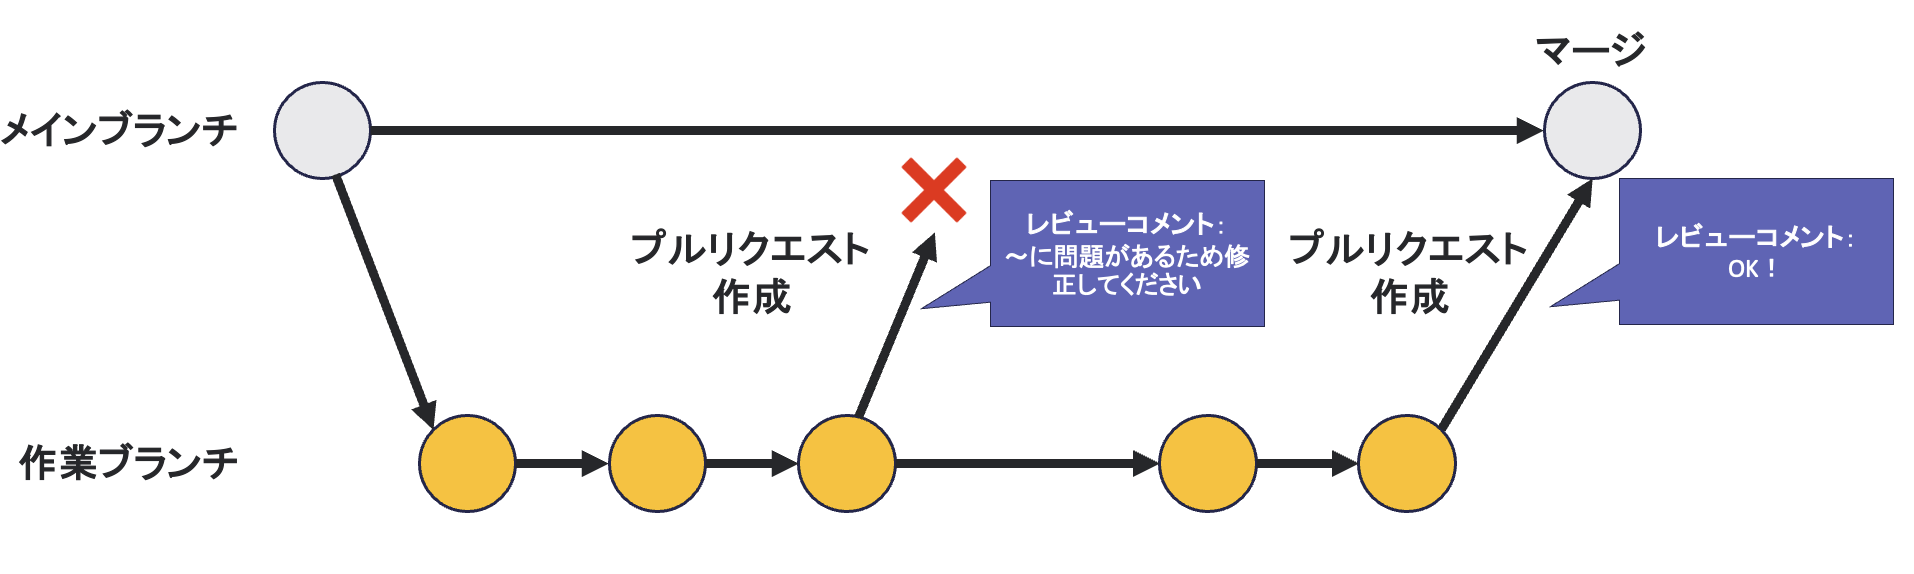
\includegraphics[width=1.0\linewidth]{@BSthesis2024_Akamatsu/Akamatsu_figs/pull-request.png}}
    \caption{変更箇所の特定方法の概略図}
    \label{fig:Insufficient_documentation}
\end{figure*}

Pull Requestは,開発者が作成したソースコードの変更を本番環境に反映する前に,その変更内容をレビューアに確認を依頼する仕組みである.実装者はまず新しい機能の追加やバグ修正のために,メインブランチから作業用ブランチを作成する.その後,作業用ブランチで必要な変更を加え,Pull Requestを作成する.レビューアは,Pull Requestで示された変更内容について,コーディング規約への準拠,バグや潜在的な問題の有無,設計の適切性,パフォーマンスへの影響,セキュリティ上の懸念などの観点からレビューを行う.問題を発見した場合はコメントを付けて修正を依頼し,実装者は指摘された箇所を修正して再度レビューを依頼する.最終的にレビューアが承認すると,変更内容がメインブランチにマージされる.

このようなコードレビューを行うことで,ソースコードのバグの混入率が低下する\cite{Vable2021Code}だけでなく,開発者間での知識伝達が促進され\cite{bacchelli2013expectations},コードの品質と保守性が向上するという利点もある.また,チーム内でのベストプラクティス(例えば,コードの再利用性を高めるためのデザインパターンの適用方法や,パフォーマンスを考慮したアルゴリズムの実装方法,セキュリティを考慮した入力値の検証方法など)の共有が進む.しかし,コードレビューにはいくつかの課題も存在する.実装者にとっては,レビュー待ち時間により開発作業が停滞し,機能のリリースが遅延するという問題がある.また,レビューアは自身の開発作業に加えてレビュー作業も行う必要があり,作業負荷の増加によって本来の開発タスクに支障が出る可能性がある.これらの問題は,プロジェクト全体のスケジュールにも影響を与え,製品のリリースの遅れにもつながりうる.また,レビューコメントの解釈に齟齬が生じた場合は,追加のコミュニケーションが必要となり,さらなる時間的コストが発生する.特に大規模なプロジェクトでは,膨大なレビュー件数の管理も大きな課題となっている.

\section{従来研究}
コードレビューの自動化に関する研究として,Tufanoらの研究\cite{tufano2022using}が挙げられる.この研究では,次の2つのタスクを対象にDeep Learningモデルによる自動化を試みている:

1つ目は,コードレビュー提出前のフィードバック生成である.開発者が提出したコード($C_s$)に対して,レビューアが指摘するであろう修正を実装したコード($C_r$)を自動生成する.これにより,開発者は正式なレビュー前に潜在的な問題点を把握できる.このタスクでは,1つのエンコーダと1つのデコーダで構成されたモデルを採用している.エンコーダは提出コード($C_s$)を入力として受け取り,ベクトル表現に変換する.デコーダはそのベクトル表現から修正後のコード($C_r$)を生成する.

2つ目は,レビューアのコメントに基づくコード修正の自動化である.開発者が提出したコード($C_s$)とレビューアのコメント($R_{nl}$)を入力とし,そのコメントに対応した修正を実装したコード($C_r$)を生成する.これにより,レビューアは具体的な修正例を開発者に示すことができる.このタスクでは,2つのエンコーダと1つのデコーダで構成されたモデルを採用している.第1エンコーダは提出コード($C_s$)を,第2エンコーダはレビューコメント($R_{nl}$)をそれぞれベクトル表現に変換する.デコーダはこれら2つのベクトル表現を組み合わせて修正後のコード($C_r$)を生成する.

これらのモデルでは,コードとコメントのベクトル化にあたり,コードの抽象化処理が用いられている.変数識別子は特別なトークン\texttt{VAR\_ID}で置き換えられる.例えば,2番目に宣言された変数は\texttt{VAR\_2}として表現される.生のソースコードに戻すため,$C_s$内の抽象化トークンと実際のトークンのマッピングが保持される(例:\texttt{VAR\_1} $\rightarrow$ \texttt{i}).この抽象化により語彙サイズを削減し,モデルの学習が行われる.

従来研究では,GitHubおよびGerritのリポジトリから約17,000件の $\langle C_s, R_{nl}, C_r \rangle$ の3つ組データを収集し,評価を行った.コードレビュー提出前のフィードバック生成タスク(提出コードから修正案を予測するタスク)では,beam searchのサイズk=1(単一の予測)の場合で3\%,k=10(上位10個の予測候補を生成)の場合で16\%の正解率を達成した.レビューアのコメントに基づくコード修正の自動化タスクでは,k=1の場合で12\%,k=10の場合で31\%の正解率を達成している.

従来研究では,コードレビューの自動化において最大31\%の正解率を達成しているものの,レビューアからのレビューコメントに含まれる情報の種類や情報量によって精度にばらつきが見られた.実際のコードレビューでは,レビューアは様々な形式や粒度でレビューコメントを記述している.このような自動コード生成の成功例と失敗例を以下に示す:

\begin{itemize}
  \item 成功例:
  \begin{figure}[H]
    \begin{center}
      \fbox{\begin{minipage}{0.95\linewidth}
        \textbf{レビューコメント:}\\
        \ttfamily\small
        Please change the variable "result" to a name that makes it clear that it is the processing result.\\
        
        \normalfont\hrule
        
        \textbf{修正前コード:}\\
        \ttfamily\small
        int result = calculateValue(); \\
        
        \normalfont\hrule
        
        \textbf{修正後コード:}\\
        \ttfamily\small
        int processResult = calculateValue(); \\
      \end{minipage}}
    \end{center}
  \end{figure}
  
  このケースでは,具体的な変更内容(resultからprocessResultへ)を明示していたため,レビューコメントが効果的であった.
  \item 失敗例:
  \begin{figure}[H]
    \begin{center}
      \fbox{\begin{minipage}{0.95\linewidth}
        \textbf{レビューコメント:}\\
        \ttfamily\small
        The variable name is not correct. \\
        
        \normalfont\hrule
        
        \textbf{修正前コード:}\\
        \ttfamily\small
        int tmp = calculateValue(); \\
        
        \normalfont\hrule
        
        \textbf{修正後コード:}\\
        \ttfamily\small
        int value = calculateValue();  // プロジェクトの命名規則に反する変数名を生成 \\
      \end{minipage}}
    \end{center}
  \end{figure}

  このケースでは,具体的な変更内容が示されいないため,モデルがレビューアが意図していたコードを生成するにはレビューコメントが不十分である.また,望ましい命名規則の例示もないため,開発者が適切な修正を行うための情報が不足している.このような抽象的なコメントでは,モデルが適切な修正を生成することは困難である.
  
\end{itemize}

このように,コメントの具体性や提供される情報量によって,モデル生成の精度に大きな差が生じることが観察されている.この知見は,モデルを用いたコード自動修正を行う上で効果的なレビューコメントの特徴を理解するための重要な示唆を与えている.

\section{動機}

本研究では,レビューコメントの特徴を分析することで,レビューアが意図していたソースコードをモデルが生成できるレビューコメントの特徴を明らかにすることを目的とする.ここで,レビューコメントの分析には適切な評価指標が必要である.

このような背景から,本研究では以下の2つの Research Question(RQ)を設定し,レビューコメントの特徴がコード生成の精度に与える影響を分析する:

\begin{itemize}
\item RQ1:\RQone
\item RQ2:\RQtwo
\end{itemize}

従来研究では,コード生成タスクの評価指標として CodeBLEU スコアが使用されているが,入力されるソースコードの規模によってスコアが大きく変動することが観察されている.例えば,大規模なコードに対する小規模な修正では,修正の質に関わらず高いスコアが付与される傾向がある.したがって,レビューコメントの特徴がコード生成の精度に与える影響を正確に分析するためには,CodeBLEU スコアを評価指標として使用する際の適切なソースコード規模を明らかにする必要がある.
そのため分析に先立ち,3章では CodeBLEU スコアが適切に評価指標として機能するソースコードの規模について分析を行う.そのうえで,4章と5章において,それぞれの RQ に対する詳細な分析を実施する.

\chapter{事前分析}\label{chap:fig-tab-exp}

\section {CodeBLEUスコア}

codeBLEUスコア\cite{ren2020codebleu}は,自然言語処理(NLP: Natural Language Processing)の分野,特にコード生成タスクにおいて使用される評価指標である.従来の機械翻訳の評価には生成データと正解データが完全一致している割合やN-gramが用いられてきた.しかし,完全一致では正解データと類似度の高いデータを生成できても十分に評価されない.また,N-gramでは単語の並び順や文の構造については評価できるが,文法的な意味や論理的な意味まで考慮できない.そこで近年では機械翻訳タスクの評価にはBLEU\cite{papineni2002bleu}スコアが用いられる.

\begin{displaymath}
\text{BLEU} = BP \cdot \exp\left(\sum_{n=1}^{N} w_n \log(p_n)\right)
\end{displaymath}

\noindent
ただし,

\begin{displaymath}
BP =
\begin{cases} 
1 & (c > r) \\ 
e^{1 - r/c} & (c \leq r)
\end{cases}
\quad
\begin{aligned}
&c: \text{生成文の長さ} \\
&r: \text{正解文の長さ}
\end{aligned}
\end{displaymath}

\vspace{1em}

\begin{displaymath}
p_n = \frac{\sum_{i} \text{生成文 }i \text{ と正解文 }i \text{ で一致した } n\text{-gram の数}}{\sum_{i} \text{生成文 }i\text{ の } n\text{-gram の総数}}
\end{displaymath}

\vspace{1em}

\begin{displaymath}
w_n = \frac{1}{N}
\end{displaymath}

BLEUスコアを採用することで部分的な一致も評価に含めることが可能になり,意味的に正しいが異なる実装も適切に評価できる.また,複数のN-gramスコアを組み合わせることで,局所的な類似性だけでなく,より広い文脈の類似性も評価できる.

BLEUスコアを用いると自然言語間の類似度を包括的に評価できるが,ソースコードを評価する際にはソースコードが持つ特徴を十分に考慮できないという課題がある.具体的には,ソースコードは自然言語に比べ使用される単語の種類が少ないため直感的な一致度よりもスコアが高くなってしまうことや,自然言語のようなシーケンシャル構造ではなくツリー構造を持っているためN-gramでは類似度を正しく評価できない.また,異なる実装方法でも同じ結果を得られるというコードの意味的同値性や,各プログラミング言語に固有のAPIの使用規則についても考慮できない.

これらのようなソースコード間の類似度を評価できない課題に対応するために,次の4つの要素を考慮した評価指標CodeBLEUスコアを用いる.

\begin{displaymath}
\text{CodeBLEU} = \alpha \cdot \text{BLEU} + \beta \cdot \text{BLEU}_{\text{weight}} + \gamma \cdot \text{Match}_{\text{ast}} + \delta \cdot \text{Match}_{\text{df}}
\end{displaymath}

\noindent
ただし,
\begin{align*}
&\alpha, \beta, \gamma, \delta: \text{重み係数(}\alpha + \beta + \gamma + \delta = 1\text{)} \\
&\text{BLEU}: \text{通常のBLEUスコア} \\
&\text{BLEU}_{\text{weight}}: \text{言語固有のキーワードに基づく重み付きBLEUスコア} \\
&\text{Match}_{\text{ast}}: \text{抽象構文木の一致率} \\
&\text{Match}_{\text{df}}: \text{データフローの一致率}
\end{align*}

CodeBLEUスコアでは,従来のBLEUスコアに加え,次の3つの指標を統合することで,ソースコード特有の性質を考慮した評価を実現している.
第一に,重み付きBLEUスコア($\text{BLEU}_{\text{weight}}$)により,プログラミング言語固有のキーワードや構文要素に対して適切な重み付けを行う.第二に,抽象構文木(AST)の一致率($\text{Match}_{\text{ast}}$)により,コードの階層的構造の類似性を評価する.第三に,データフロー分析に基づく一致率($\text{Match}_{\text{df}}$)により,変数の定義や使用パターンなど,プログラムの意味的な等価性を評価する.
これらの指標に対して重み係数(α,β,γ,δ)を設定することで,評価対象やタスクの特性に応じた柔軟な評価が可能となる.この結果,CodeBLEUスコアは,プログラミング言語特有の構文規則,構造的特徴,および意味的等価性を総合的に考慮した評価指標として機能する.


\section {CodeBLEUスコアの問題点}
前節で述べたように,CodeBLEUスコアは従来のBLEUスコアにプログラミング言語特有の評価指標を組み込むことで,ソースコード生成タスクにおいてより適切な評価を可能とした.しかしながら,CodeBLEUスコアには入力されるソースコードの規模に依存してスコアが変動するという問題が存在する.この課題を具体的に示す従来研究の結果の事例として,図\ref{fig:low-score}と図\ref{fig:high-score}の比較が挙げられる.

\begin{figure}[H]
    \begin{center}
        \fbox{\begin{minipage}{0.95\linewidth}
            //CODEBLEU score: 0.057\\
            
            \textbf{//修正前コード:}\\
            \textbf{//ソースコード総行数:5行}\\
            \ttfamily\small
            protected GenericRecord readEntity()\\
            \hspace{4ex}throws IOException\\
            \{\\
            \hspace{4ex}return readRecord();\\
            \}\\
            
            \normalfont\hrule
            
            \textbf{//レビューコメント:}\\
            another level method redirection if else is in it
        \end{minipage}}
        \caption{CodeBLEU scoreが低い修正ソースコード}
        \label{fig:low-score}
    \end{center}
\end{figure}

\begin{figure}[H]
   \begin{center}
       \fbox{\begin{minipage}{0.95\linewidth}
           //CODEBLEU score: 0.997\\
           
           \textbf{//修正前コード:}\\
           \textbf{//ソースコード総行数:55行}
           
           \ttfamily\small
           public StringBuffer generate(...) throws\\
           GenerationException \{\\
           \hspace{4ex}final Messager messager = ...\\
           \}\\
           
           messager.printMessage(Diagnostic.Kind.NOT\\
           E, ""\\
           \hspace{4ex}Successfully generated code\\
           \hspace{4ex}for ["" + className + ""]\\
           "");\\
           processingContext.addRule(ruleId,\\
           \hspace{4ex}ProcessingRule.TYPE.DOCKING,\\
           \hspace{4ex}sw.getBuffer());\\
           return null;\\
           \}\\
           
           \normalfont\hrule
           
           \textbf{//レビューコメント:}\\
           hey @pefernan , this one... is a typo
       \end{minipage}}
       \caption{CodeBLEU scoreが高い修正ソースコード}
       \label{fig:high-score}
   \end{center}
\end{figure}

図\ref{fig:low-score}は,入力されたソースコード規模は小さいが大きな変更を求められている事例である.レビューアからの指摘で,条件付きではあるが新たなメソッドを追加することが指示されており,大きな変更が求められている.入力されたソースコードからは大きく変更が加えられることになり CodeBLEU スコアが低くなることは必然である.一方で図\ref{fig:high-score}では,55行のソースコードが入力され,レビューアからの指摘は誤字の指摘であり,修正箇所が小さい事例である.従来研究の結果全体のうちCodeBLEU スコアの高いソースコードのレビュー指摘を確認したところ,修正規模が小さいケースが多数存在していた.以上より,コードレビューの自動修正においては,入力するソースコード規模別の評価,および修正規模に応じた評価指標の改善が必要であると考える.

\section {事前分析の目的}
本章では,コード自動修正モデルの評価指標であるCodeBLEUスコアを適切に使用するために,評価対象とすべきソースコードの規模を明らかにすることを目的とする.前節で述べたように,CodeBLEUスコアは入力されるソースコードの規模により結果が大きく変動する可能性があり,特に大規模なソースコードに対する小規模な修正では不当に高いスコアが,小規模なソースコードに対する大規模な修正では不当に低いスコアが付与される傾向にある.そこで本研究では,コードレビューのデータセットを用いて,CodeBLEUスコアが修正の質を適切に評価できるソースコードの規模を定量的に分析する.これにより,コード自動修正モデルの評価において,CodeBLEUスコアを適切に活用するためのソースコードの規模を確立することを目指す.


\section {データセット}
本分析では従来研究で行われた分析結果を対象に分析を行った.従来研究ではGitHubおよびGerritリポジトリからコードレビュー関連のデータを収集されていた.

\begin{itemize}
    \item プロジェクト選定条件:
    \begin{itemize}
        \item Pull Request数が50件以上.
        \item 10人以上の貢献者および10個以上のStarを持つプロジェクト.
    \end{itemize}
    \item データ構造:
    \begin{itemize}
        \item 各データは以下の3つの要素で構成されている $\langle m_s, c_{nl}, m_r \rangle$:
        \begin{itemize}
            \item $m_s$: 提出されたメソッド.
            \item $c_{nl}$: レビューアによる変更提案コメント.
            \item $m_r$: 修正後のメソッド.
        \end{itemize}
        \item 合計167,799件収集されている.
    \end{itemize}
\end{itemize}

\section {分析準備}

分析の準備として,以下の手順を行った.

\begin{enumerate}
   \item データセットから入力コードのノード数と変更ノード数の外れ値を除去する.具体的には,それぞれの四分位範囲(IQR)を計算し,第1四分位数(Q1)から四分位範囲の1.5倍を引いた値より小さい値,または第3四分位数(Q3)に四分位範囲の1.5倍を加えた値より大きい値を外れ値として除去する.

   \item 入力コードのノード数とCodeBLEUスコアの関係性を分析するため,外れ値を除去した後のデータセットを入力コードのノード数に基づいて4つのグループに分割する.具体的には,ノード数の四分位数(Q1,Q2(中央値),Q3)を基準として,以下の4グループに分類する.
   \begin{itemize}
       \item グループ1:Q1未満のノード数
       \item グループ2:Q1以上Q2未満のノード数
       \item グループ3:Q2以上Q3未満のノード数
       \item グループ4:Q3以上のノード数
   \end{itemize}
\end{enumerate}


\section{分析手順}

\subsection {変更箇所の特定}

\begin{figure*}[ht]
    \centerline{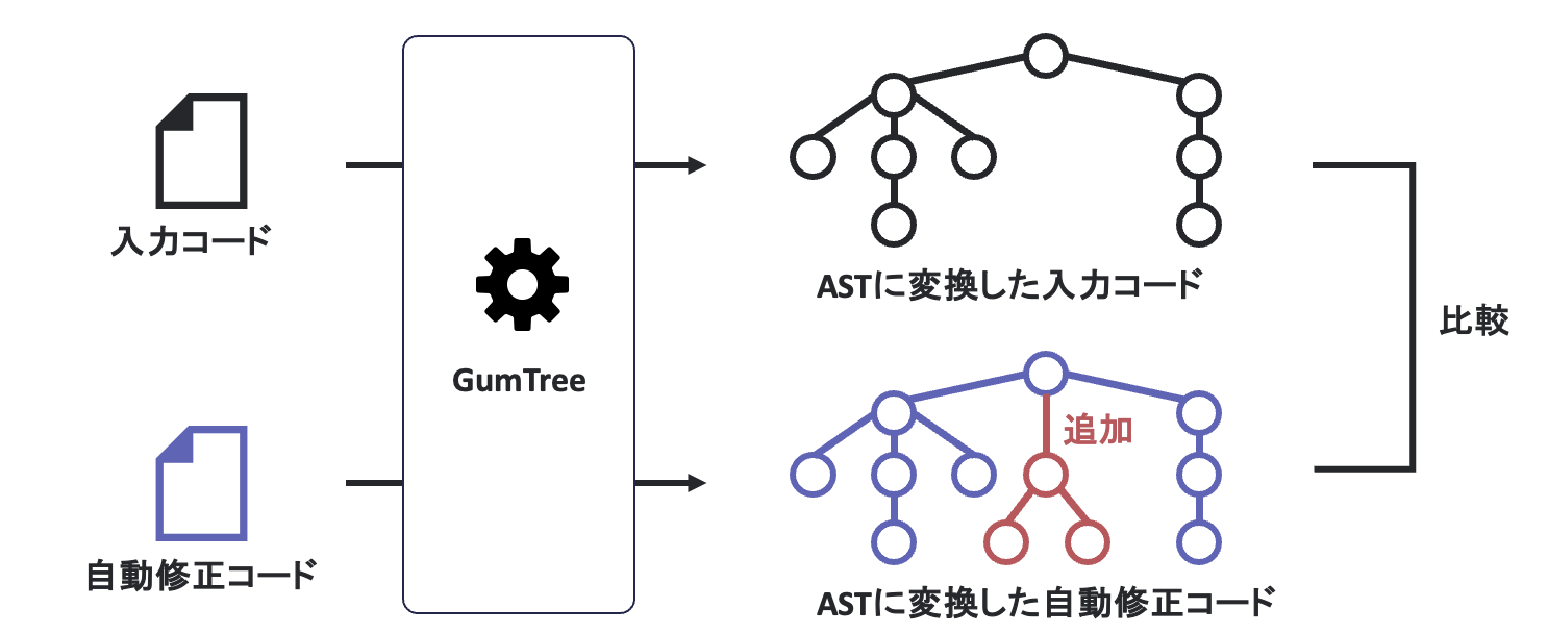
\includegraphics[width=1.0\linewidth]{@BSthesis2024_Akamatsu/Akamatsu_figs/AST.pdf}}
    \caption{変更箇所の特定方法の概略図}
    \label{fig:Insufficient_documentation}
\end{figure*}
図\ref{fig:Insufficient_documentation}に示すように,提出されたメソッド($m_s$)と修正後のメソッド($m_r$)の変更箇所を特定するために,抽象構文木(AST: Abstract Syntax Tree)の差分分析を行う.差分分析にはGumTree\cite{DBLP:conf/kbse/FalleriMBMM14}を使用し,次の手順で変更箇所の特定を行った.

まず,提出されたメソッド($m_s$)と修正後のメソッド($m_r$)それぞれに対してASTを生成する.次に,GumTreeを用いて2つのAST間の差分を抽出する.GumTreeは,新しいノードを追加する操作(INSERT),既存ノードを削除する操作(DELETE),ノードの値を更新する操作(UPDATE),そしてノードの位置を変更する操作(MOVE)の4種類の操作を特定する.最後に,抽出された差分情報から変更が行われた箇所とその種類を特定し,変更ノード数を算出する.

この手法により,変更差分を定量的に算出し,入力コード全体のノード数と比較する.

\section{分析結果}



\subsection {分析1: グループ間のCodeBLEUスコアの分布の差異}

\begin{table}[h]
   \centering
   \caption{グループ間のマン・ホイットニーU検定のp値}
   \label{tab:mann-whitney}
   \begin{tabular}{l|cccc}
       \hline
       p値 & グループ1 & グループ2 & グループ3 & グループ4 \\
       \hline
       グループ1 & - & p値 \verb|<| 0.01 & p値 \verb|<| 0.01 & p値 \verb|<| 0.01 \\
       グループ2 & - & - & p値 \verb|<| 0.01 & p値 \verb|<| 0.01 \\
       グループ3 & - & - & - & p値 \verb|<| 0.01 \\
       グループ4 & - & - & - & - \\
       \hline
   \end{tabular}
\end{table}

各グループ間でCodeBLEUスコアの分布に統計的な差があるかを検証するため,マン・ホイットニーのU検定を実施した.有意水準は0.05に設定し,全てのグループの組み合わせで検定を行った結果,すべての組み合わせにおいてp値が有意水準を下回った(p \verb|<| 0.05).これは,入力コードのノード数の違いによってCodeBLEUスコアの分布が有意に異なることを示している.

表\ref{tab:mann-whitney}に示すように,全ての組み合わせにおいてp値は0.05を大きく下回っており,各グループ間のCodeBLEUスコアの分布には統計的に有意な差があることが確認された.

\subsection {分析2: 同一タスクにおけるコード量の影響}
\begin{figure}[h]
    \centering
    \fbox{\begin{minipage}{0.95\linewidth}
        \textbf{//コード例1} \\
        \textbf{//CODEBLEU score: 0.750} \\
        \textbf{//入力コードのノード数: 5} \\
        \textit{(//赤色の部分は変更箇所を示す)} \\
        
        \ttfamily\small
public String getRpmRevision() \{\\
\hspace{4ex}return this.\textcolor{red}{rpmRevison};\\
\}\\

        \normalfont\hrule
        //レビューコメント: typo above, be: return this.rpmRevision;
    \end{minipage}}

    \vspace{4mm}

    \fbox{\begin{minipage}{0.95\linewidth}
        \textbf{//コード例2} \\
        \textbf{//CODEBLEU score: 0.996} \\
        \textbf{//入力コードのノード数: 80} \\
        \textit{(//赤色の部分は変更箇所を示す)} \\
        
        \ttfamily\small
public StringBuffer generate(\\
\hspace{4ex}final String packageName,\\
\hspace{4ex}final PackageElement packageElement,\\
\hspace{4ex}final String className,\\
\hspace{4ex}final Element element,\\
\hspace{4ex}final ProcessingEnvironment\\
\hspace{4ex}processingEnvironment) throws GenerationException \{\\
\hspace{4ex}final Messager messager =\\
\hspace{8ex}processingEnvironment.getMessager();\\
\hspace{4ex}Messager.printMessage(Diagnostic.Kind.NOTE,\\
\hspace{8ex}"Starting code \textcolor{red}{generation} for [" + className + "]");\\
\hspace{4ex}// ... (42行省略)\\
\}\\

        \normalfont\hrule
        //レビューコメント: hey @pefernan , this one... is a typo
    \end{minipage}}
    \caption{同一タスク(タイプミス)における入力コード量の違いによるCodeBLEUスコアの比較}
    \label{fig:code-comparison}
\end{figure}

同一タスク(タイプミス)に対して,入力コードの規模が異なる場合のCodeBLEUスコアを比較した.具体的には,変更ノード数が1で同一のタスク(タイプミスの修正)である2つのケースを分析した.その結果,入力コードのノード数が5の場合はCodeBLEUスコアが0.750であったのに対し,ノード数が80の場合は0.996と大幅に高いスコアを示した.これは,同じ種類の修正であっても,入力コードの規模が大きくなるとCodeBLEUスコアが高くなる傾向があることを示している.

\subsection {分析3: ノード数別の修正規模とスコアの関係}
図\ref{fig:node-scores}は,入力コードのノード数によって分類した4つのグループにおける,変更ノード数とCodeBLEUスコアの分布を示す.横軸は変更ノード数を5刻みで区切ったグループを表し,縦軸は各グループにおけるCodeBLEUスコアの分布を箱ひげ図で表している.入力コードのノード数は3〜233の範囲を4分位で分割し,3〜25,25〜45,45〜75,75〜233の4グループとした.

\begin{figure}[h]
   \centering
   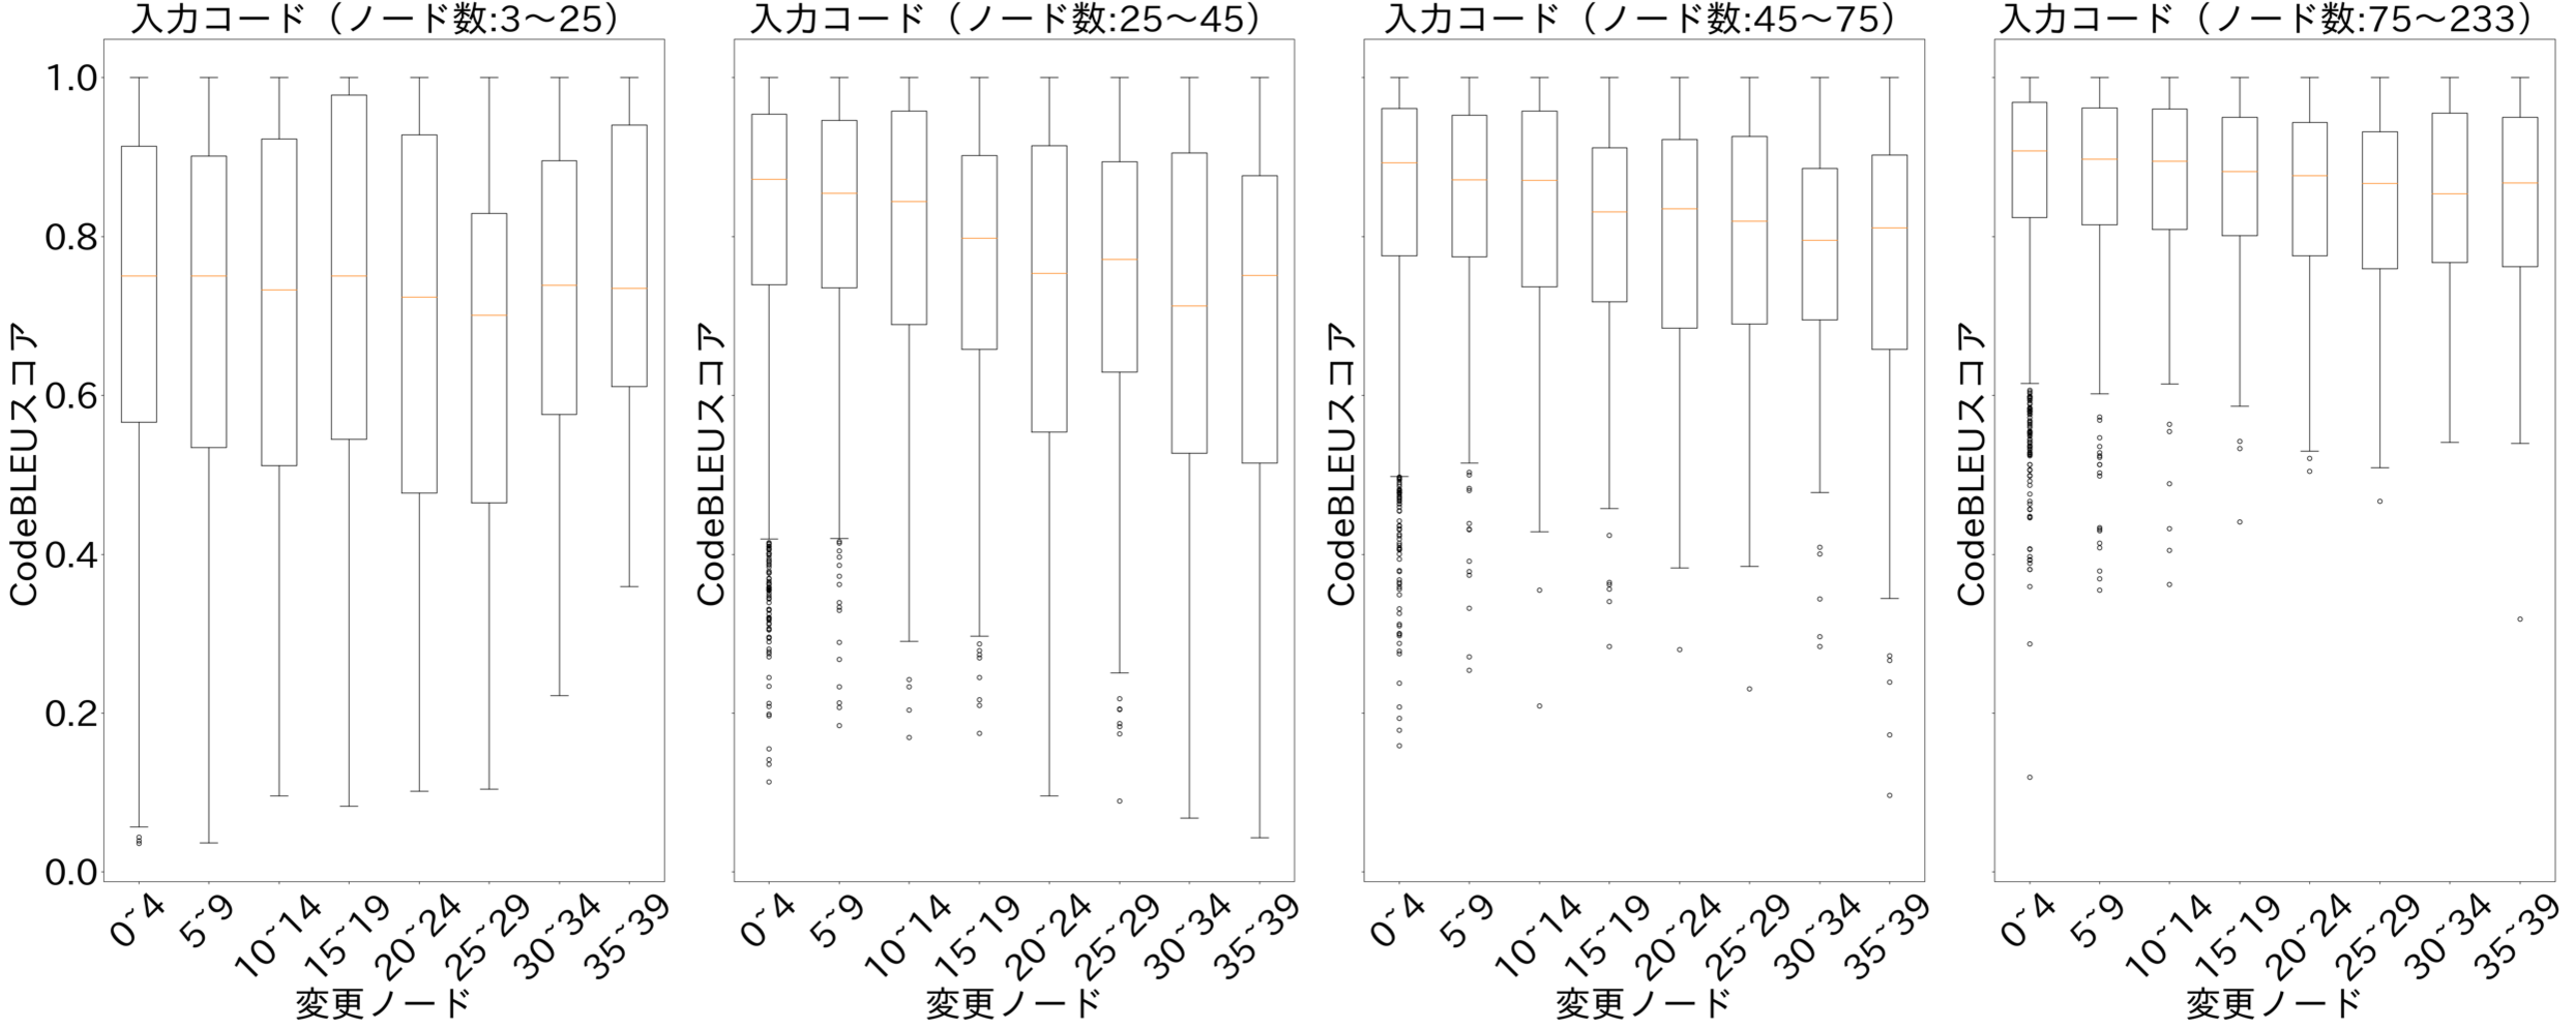
\includegraphics[width=1.0\linewidth]{@BSthesis2024_Akamatsu/Akamatsu_figs/nodescores.pdf}
   \caption{入力コードのノード数別のCodeBLEUスコアの分布}
   \label{fig:node-scores}
\end{figure}

特筆すべき分析結果として,次の2点が挙げられる:

\begin{enumerate}
   \item 入力コードのノード数が75〜233(第3四分位数から最大値)の場合,変更ノード数が増加してもCodeBLEUスコアは0.8前後の高い値を維持している.これは,入力コード全体に対する変更部分の割合が相対的に小さいため,変更の規模に関わらず全体としての一致率が高くなってしまうことを示している.つまり,この範囲のノード数では,CodeBLEUスコアが修正の質を適切に評価できていない可能性がある.
   
   \item 入力コードのノード数が25〜45(第1四分位数から中央値)の場合,変更ノード数の増加に伴いCodeBLEUスコアが単調に減少する傾向が見られた.これは,コードの変更規模が大きくなるにつれて修正の難易度が上がり,生成精度が低下することを適切に反映している.この範囲のノード数では,CodeBLEUスコアが修正の質を適切に評価できていると考えられる.
\end{enumerate}

以上の分析結果から,CodeBLEUスコアを評価指標として使用する際は,入力コードのノード数が25〜45の範囲にあるケースを対象とすることで,より信頼性の高い評価が可能であることが示唆された.一方で,ノード数が75を超えるような大規模なコードに対しては,CodeBLEUスコアが実際の修正の質を反映していない可能性があり,評価指標としての使用には注意が必要である.これらの知見を踏まえ,以降の章では入力コードのノード数が25〜45の範囲にあるデータセットを用いて分析を行う.この範囲のデータセットを用いることで,CodeBLEUスコアによる評価の信頼性を確保し,より正確な分析結果を得ることを目指す.


\chapter{RQ1:\RQone}\label{chap:fig-tab-exp}
\section{概要}
本章では,レビューアが指摘したソースコードを自動生成するために必要なレビューコメントの情報の種類を明らかにする.

従来研究では,レビューコメントに基づくコード生成モデルの精度にばらつきがあることが示されているが,どのような情報の種類が自動生成の精度向上に寄与するかは詳細に分析されていない.この課題に対処するため,本研究ではレビューコメントの内容を体系的に分類するラベル付けのアプローチを採用する.具体的には,レビューコメントの情報を「コンテキスト」と「修正依頼方法」という2つの観点からラベル付けを行う.コンテキストではリファクタリング,バグ,パフォーマンスといった修正の種類を,修正依頼方法ではエラー内容の提示,再現方法の提示,具体的な修正方法の提示といった指摘方法を分類する.このラベル付けにより,レビューコメントに含まれる情報の特徴を定量的に分析することが可能となる.

本研究では,従来研究でGitHubおよびGerritから収集されたレビューコメントに対してこのラベル付けを実施し,各情報の種類とコード生成モデルの精度の関係性を分析する.この分析を通じて,高精度なコード生成を実現するために必要なレビューコメントの特性を明らかにすることを目指す.

\section{分析手法}


\subsection {データセット}
本分析では,3章と同じく従来研究で行われた分析結果を対象に分析を行った.

\begin{itemize}
    \item プロジェクト選定条件:
    \begin{itemize}
        \item Pull Request数が50件以上.
        \item 10人以上の貢献者および10個以上のStarを持つプロジェクト.
    \end{itemize}
    \item データ構造:
    \begin{itemize}
        \item 各データは以下の3つの要素で構成されている $\langle m_s, c_{nl}, m_r \rangle$:
        \begin{itemize}
            \item $m_s$: 提出されたメソッド.
            \item $c_{nl}$: レビューアによる変更提案コメント.
            \item $m_r$: 修正後のメソッド,
        \end{itemize}
        \item 合計167,799件収集されている.
    \end{itemize}
\end{itemize}

\subsection{事前処理}
\begin{figure}[htbp]
    \centering
    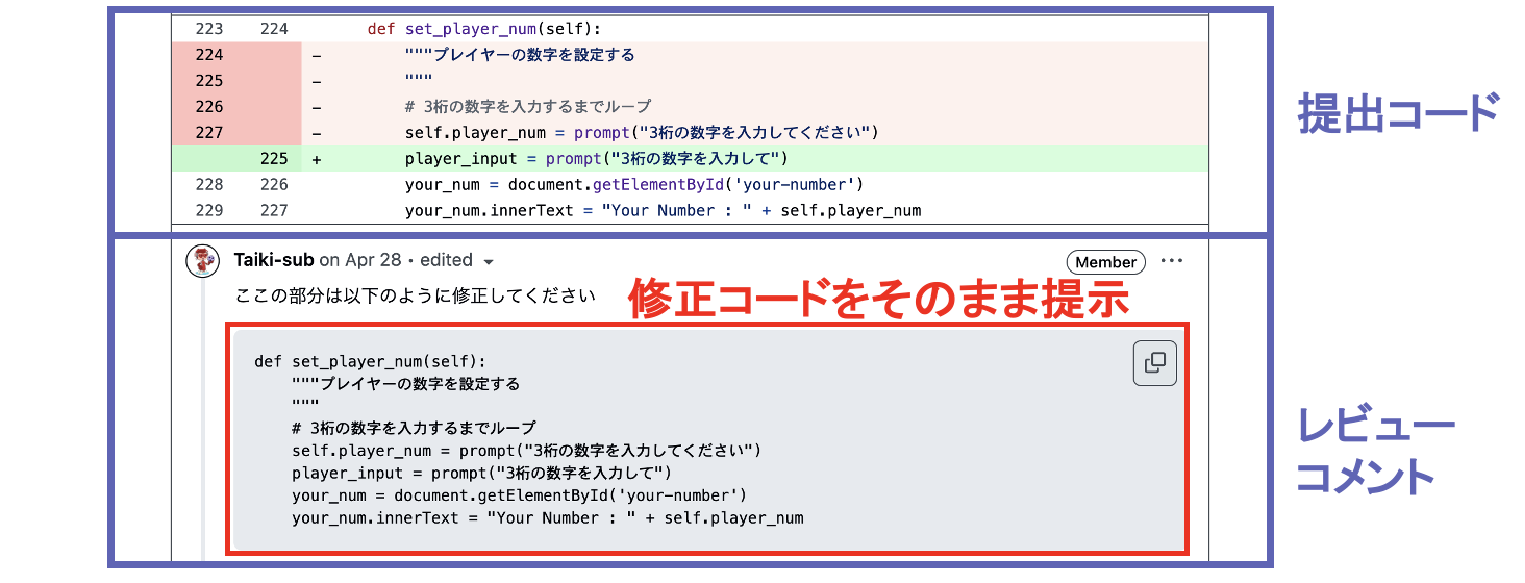
\includegraphics[width=0.8\linewidth]{@BSthesis2024_Akamatsu/Akamatsu_figs/review_comment.pdf}
    \caption{レビューアが修正コードを直接提供するレビューコメントの例}
    \label{fig:review-comment-example}
\end{figure}
分析に先立ち,収集したデータセットに対して以下の事前処理を行った.3章で述べたように,CodeBLEUスコアを評価指標として使用する際は,入力コードのノード数が25〜45の範囲にあるケースを対象とすることで,より信頼性の高い評価が可能であることが示唆された.そのため,本分析では入力コードのノード数が25〜45の範囲にあるデータのみを抽出し,分析対象とした.これにより,CodeBLEUスコアによる評価の信頼性を確保し,より正確な分析結果を得ることを目指した.

次に,レビューコメントの内容を精査した.レビューコメントの中には,図\ref{fig:review-comment-example}に示すように,修正方法や修正理由の説明ではなく,修正後のコードそのものを提供している場合が存在する.このようなコメントは,レビューアが開発者の役割まで果たしているため,本研究の目的と逸脱している.またレビューアが意図した修正の背景や理由を理解することができず,レビューコメントから得られる情報の種類を適切に分析することができない.そのため,レビューコメントと修正コードとの文字列一致度を計算し,一致度が高いコメント,すなわち修正コードをそのまま含むコメントは分析対象から除外した.これにより,レビューアの意図や修正の理由が明確に記述されたコメントのみを分析対象とすることにした.

最後に,統計的な有意性を確保するためのサンプリングを行った.収集したデータセット全体(16,780件)に対して,統計的に有意な分析を行うために必要なサンプル数を算出した.具体的には,信頼水準95\%,許容誤差5\%の条件下で必要なサンプル数を計算し,375件のレビューコメントを無作為に抽出してラベル付けを行った.

これらの事前処理により,CodeBLEUスコアによる評価の信頼性を確保し,レビューコメントの本質的な情報を分析対象とし,かつ統計的な有意性を持つデータセットを準備することができた.


\subsection{ラベル付け}
レビューコメントに含まれる情報の種類を分析するため,各レビューコメントに対して2つの観点からラベル付けを行った.
1つ目の観点はコンテキストである.レビューアが指摘している修正の背景や目的を分類するため,以下の3つのカテゴリを設定した:
\begin{itemize}
\item リファクタリング:コードの可読性や保守性を向上させるための修正
\item バグ:プログラムの不具合や意図しない動作の修正
\item パフォーマンス:実行速度やメモリ使用量などの性能に関する修正
\end{itemize}
2つ目の観点は修正依頼方法である.レビューアがどのような形で修正を依頼しているかを分類するため,以下の3つのカテゴリを設定した:
\begin{itemize}
\item エラーの内容の提示:発生している問題や不具合の内容を説明
\item 再現方法の提示:問題が発生する条件や手順を説明
\item 具体的な修正方法の提示:どのように修正すべきかの具体的な方法を説明
\end{itemize}
なお,1つのレビューコメントに複数の情報が含まれる場合は,主たる情報に基づいてラベル付けを行った.

\section{結果}
レビューコメントの分析結果について,コンテキストの観点から得られたCodeBLEUスコアの分布を図\ref{fig:context-score}に示す.
\begin{figure}[htbp]
\centering
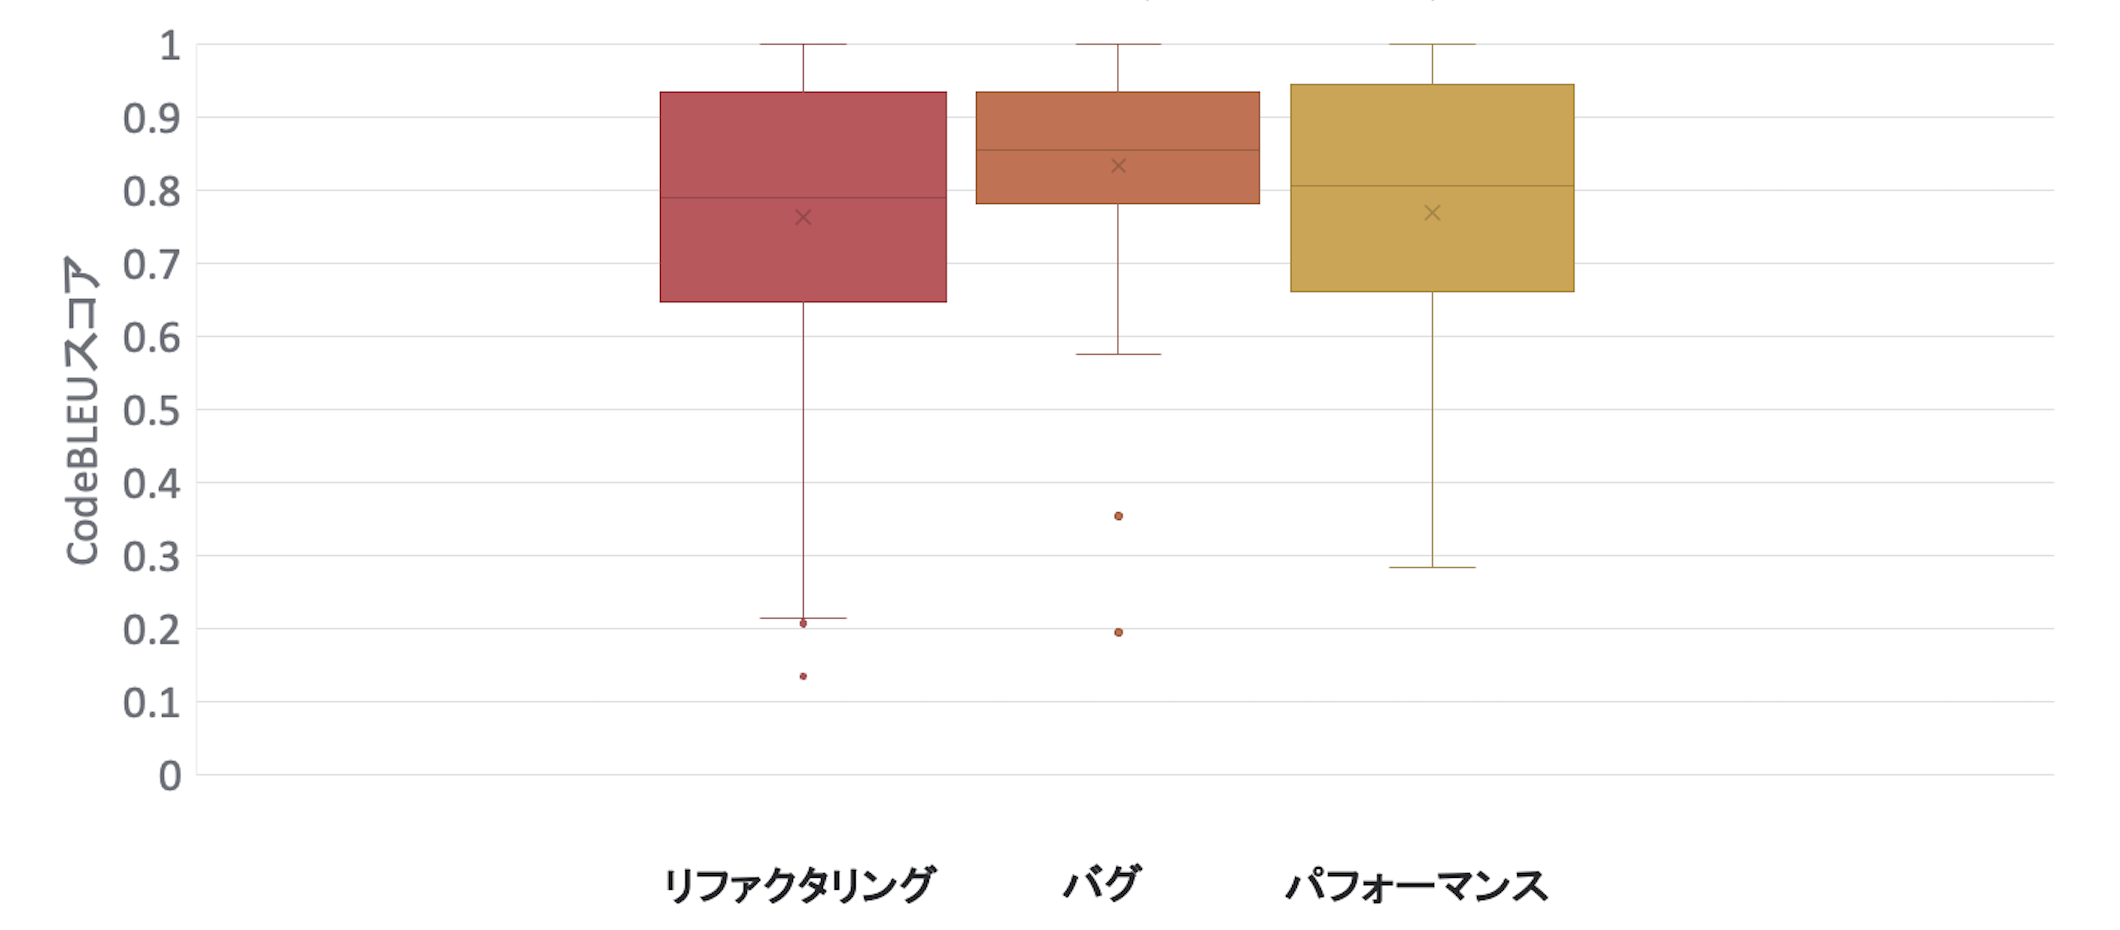
\includegraphics[width=0.8\linewidth]{@BSthesis2024_Akamatsu/Akamatsu_figs/rq1_result02_03.png}
\caption{コンテキストの種類別によるCodeBLEUスコアの分布比較}
\label{fig:context-score}
\end{figure}
まず,コンテキストの観点から見ると,リファクタリング,バグ,パフォーマンスの3種類のコンテキスト間でCodeBLEUスコアの分布に大きな差は見られなかった.各コンテキストのスコアの中央値はそれぞれ0.78,0.83,0.77程度であり,四分位範囲(IQR)も同程度の広がりを示している.特に,バグに関するコンテキストでは若干高いスコアを示す傾向があったものの,いずれのラベル間でも,統計的有意差は確認されなかった(p \textgreater 0.05).このことから,修正の背景や目的の違いは,コード生成モデルの精度に大きな影響を与えないことが示唆された.また,全てのコンテキストにおいて,外れ値として0.20〜0.40程度の低いスコアを示すケースが観察されたが,これらは全体の5\%未満であり,モデルの一般的な性能を評価する上では無視できる範囲であると判断した.
一方,修正依頼方法の観点からの分析結果を図\ref{fig:method-score}に示す.
\begin{figure}[htbp]
\centering
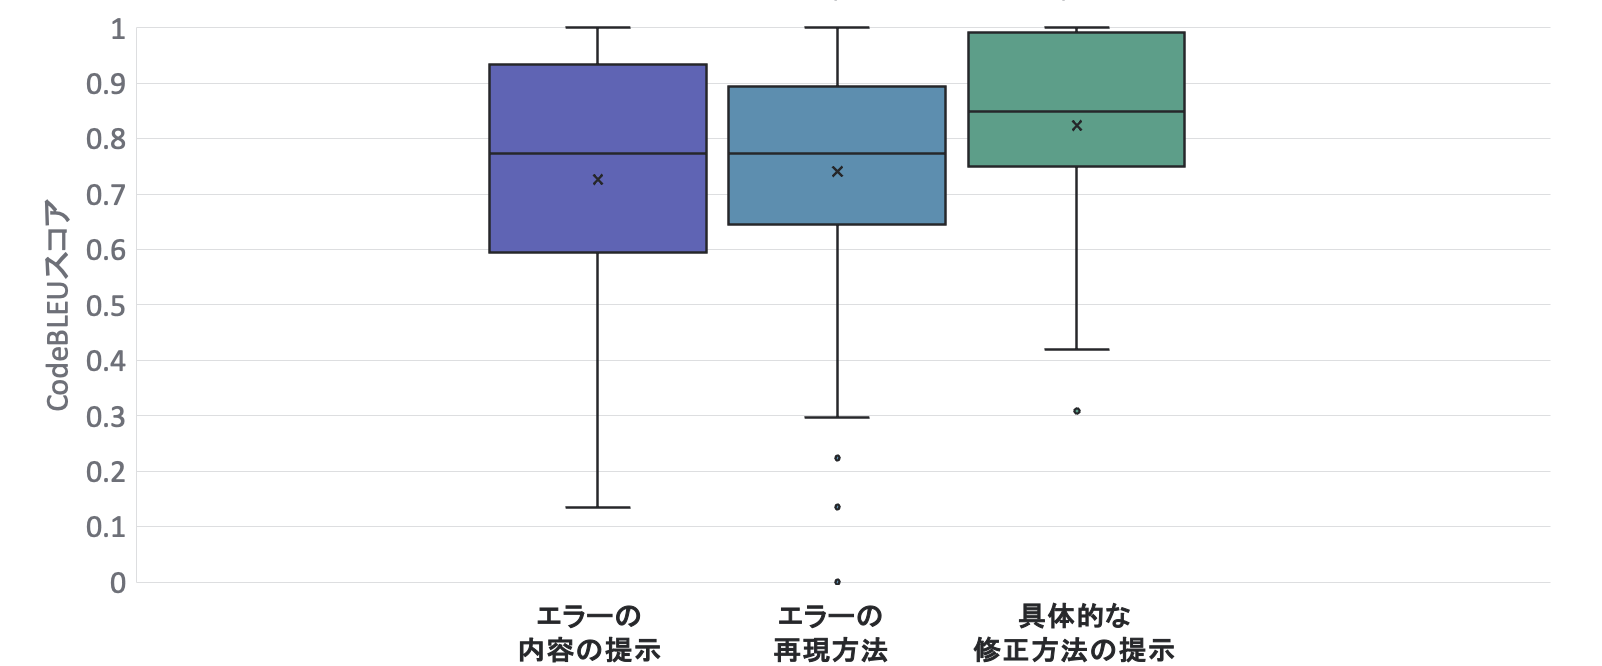
\includegraphics[width=0.8\linewidth]{@BSthesis2024_Akamatsu/Akamatsu_figs/rq1_result03_03.png}
\caption{修正依頼方法の違いによるCodeBLEUスコアの分布比較}
\label{fig:method-score}
\end{figure}
具体的な修正方法の提示が最も高いCodeBLEUスコアを示し(中央値:0.85,IQR:0.75-0.95),次いでエラーの再現方法(中央値:0.74,IQR:0.65-0.89),エラーの内容の提示(中央値:0.72,IQR:0.60-0.93)という順序となった.特筆すべき点として,具体的な修正方法を提示するコメントでは,スコアの分布がより上位に集中しており,外れ値も他の方法と比較して少ないことが確認された.これは,具体的な修正方法を提示することで,モデルがより安定して高精度なコード生成を実現できることを示唆している.
さらに,修正依頼方法とコンテキストを組み合わせた9つのカテゴリ(3×3)での分析結果を図\ref{fig:matrix-score}に示す.
\begin{figure}[htbp]
\centering
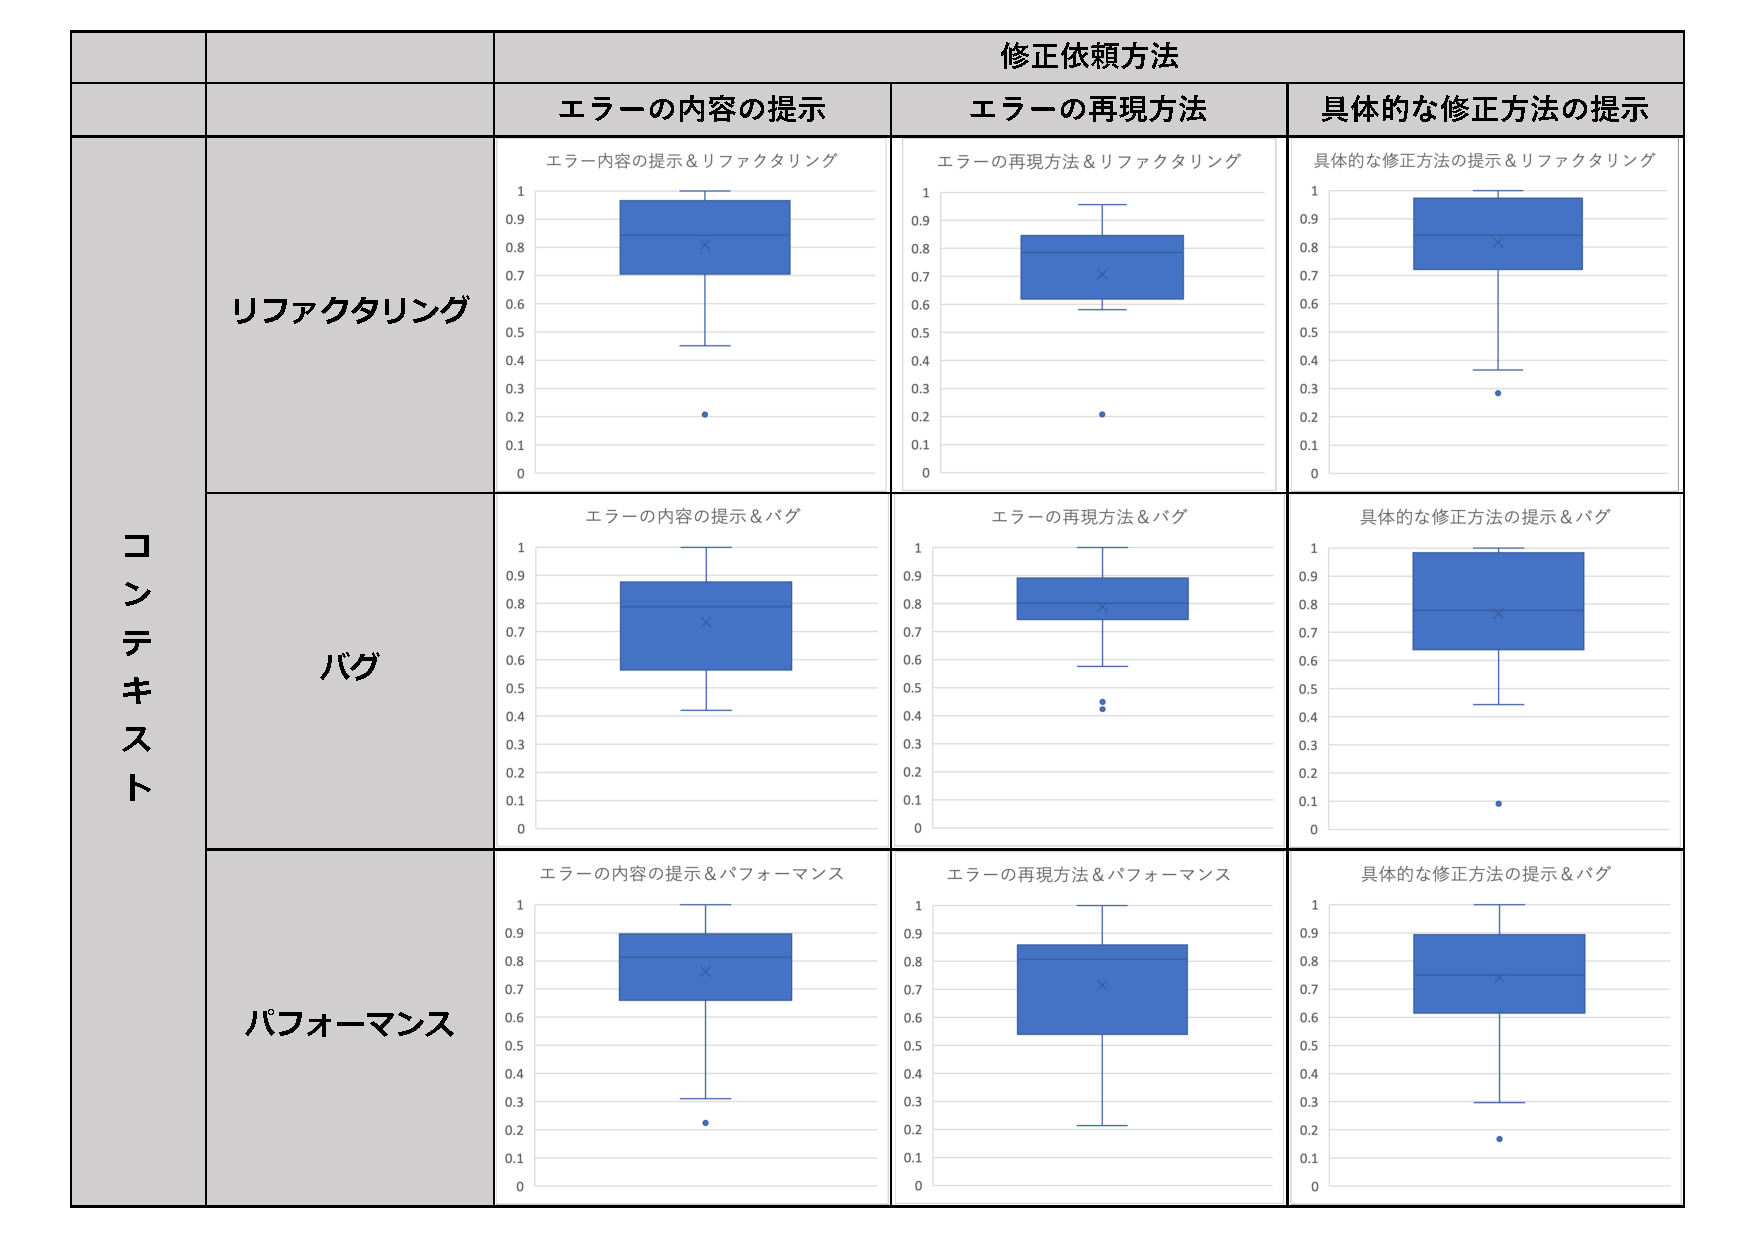
\includegraphics[width=0.9\linewidth]{@BSthesis2024_Akamatsu/Akamatsu_figs/rq1_result01.pdf}
\caption{修正依頼方法とコンテキストの組み合わせによるCodeBLEUスコアの分布}
\label{fig:matrix-score}
\end{figure}
例えば,「リファクタリング×具体的な修正方法の提示」や「バグ×エラーの再現方法」といった組み合わせごとにCodeBLEUスコアの分布を分析したが,カテゴリ間で統計的有意差は確認されなかった(p \textgreater 0.05).この結果は,コード生成の精度に最も影響を与えるのは修正依頼方法であり,コンテキストの違いによる影響は限定的であることを示している.また,この分析により,修正依頼方法の効果はコンテキストに依存せず,普遍的であることも示唆された.
これらの結果から,ソースコードを自動生成する際は,コンテキストの種類に関わらず,具体的な修正方法を提示するレビューコメントが最も効果的であることが明らかになった.また,エラーの再現方法や内容の提示だけでは,モデルが適切な修正を推論することが比較的困難であることも示された.


\chapter{RQ2:\RQtwo}\label{chap:fig-tab-exp}
\section{概要}
本章では,レビューアが指摘したソースコードを自動生成するために必要なレビューコメントの情報量を明らかにする.
従来研究では,レビューコメントに基づくコード生成モデルの精度にばらつきがあることが示されているが,自動生成の精度向上に必要な情報量については詳細な分析が行われていない.そこで本研究では,GitHubのPull Requestに含まれる追加情報(コミットメッセージ,ラベルなど)を用いてレビューコメントを段階的に拡張し,各段階での自動生成コードの精度を比較することで,効果的なコード生成に必要な情報量を定量的に分析する.


\section{データセット}
本分析では,GitHubから収集したPull Request(PR)とそれに関連するデータを対象とする.データ収集にあたっては,以下の条件を満たすPRを抽出した:
\begin{itemize}
\item マージされたJavaファイルを含むこと
\item マージされたJavaファイルに対するレビューコメントが存在すること
\item 対象のJavaファイルがそのPR内で変更されていること
\end{itemize}
データの収集では,GitHubのリポジトリをStar数の降順で検索し,上記条件を満たす1,808件のPRから,合計7,860件のレビューコメントを収集した.各PRについて,以下の情報を取得した:
\begin{itemize}
\item 自動コード修正モデルに入力する情報
\begin{itemize}
\item 変更前のJavaファイル:修正前の状態を示すソースコード
\item 変更後のJavaファイル:レビューコメントを受けて修正された後のソースコード
\item レビューコメント:レビューアによる指摘や提案内容
\end{itemize}
\item レビューコメントを拡張するためのPRに関するデータ
\begin{itemize}
\item PRタイトル:変更内容を要約したタイトル
\item PR Description:変更の詳細な説明や背景情報
\item ブランチ名:変更が行われたブランチの名称
\item ファイル名:対象となるJavaファイルの名称
\end{itemize}
\end{itemize}
第3章での分析結果から,CodeBLEUスコアによる評価の信頼性を確保するためには,入力コードのノード数が25〜45の範囲にあるデータを対象とすることが望ましい.そこで本分析では,収集した7,860件のレビューコメントから,入力コードのノード数が25〜45の範囲にあるデータのみを抽出し,最終的に7,079件のレビューコメントを分析対象とした.これにより,CodeBLEUスコアによる評価の信頼性を確保し,より正確な分析結果を得ることを目指す.

\section{分析手法}
レビューコメントに必要な情報量を分析するために,以下の手順で分析を行った.

\if0
\subsection{データ整形}
まず,収集したデータから分析に適した形式へのデータ整形を行った.具体的には,以下の処理を実施した:

\begin{itemize}
    \item レビューコメントが付与されている箇所を関数単位で抽出
    \item 自動修正ツールの入力形式に合わせて,Javaファイルとレビューコメントを結合
\end{itemize}
\fi

\begin{figure}[htbp]
\centering
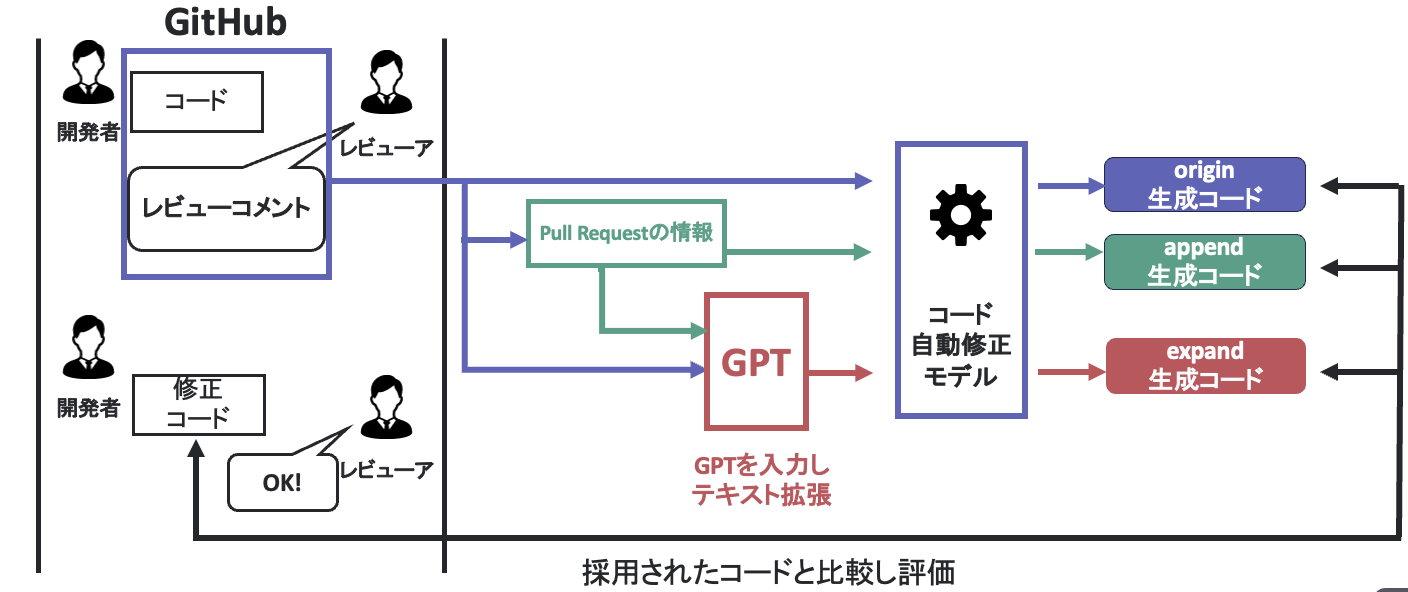
\includegraphics[width=0.9\linewidth]{@BSthesis2024_Akamatsu/Akamatsu_figs/rq2_method_02.png}
\caption{RQ2分析方法の概略図}
\label{fig:matrix-score}
\end{figure}

図\ref{fig:matrix-score}に示すように,コード自動修正モデルに与える入力情報を3段階に分けて実験を実施した.

1つ目のアプローチでは,GitHubから取得した基本的なレビューコメントとソースコードのみをコード自動修正モデルに入力し,修正コードを生成した.このアプローチで生成されたコードをorigin生成コードと呼ぶ.これをベースラインとして設定し,最小限の情報による修正精度を評価した.

2つ目のアプローチでは,基本のレビューコメントにPull Requestから得られる追加情報を機械的に連結して入力とした.具体的には,変更前のJavaファイル,ファイルパス,Pull Requestのタイトル,Pull Requestの説明文,およびブランチ情報(変更元ブランチと変更先ブランチ)を単純に結合し,一つの入力文として与える.このように情報を機械的に連結して生成されたコードをappend生成コードと呼ぶ.これにより入力情報量は増加するが,情報間の関係性は保持されたままとなる.

3つ目のアプローチでは,基本のレビューコメントと2つ目のアプローチで使用したPull Request情報をGPT-4モデルに入力し,より自然な形で文脈を補完した拡張レビューコメントを生成した.GPT-4へのリクエストには以下のパラメータを設定した:モデルにはgpt-4o-miniを指定し,temperatureは0.7に設定した.GPTへの入力は以下の構造化されたプロンプトとして与えた.

\begin{figure}[ht]
        \begin{lstlisting}[basicstyle=\ttfamily\small,
                          frame=single,
                          breaklines=true,
                          numbers=none,
                          backgroundcolor=\color{gray!10},
                          captionpos=b]
REQUIREMENTS:
  Review Comment: [レビューコメント]
  Context:
    - code: [修正前コード]
    - File: [ファイルパス]
    - PR Title: [PRタイトル]
    - PR Description: [PR説明文]
    - Branch: [変更元ブランチ] -> [変更先ブランチ]

Based on this information, please expand the review comment by providing additional context and explanations.
        \end{lstlisting}
    \caption{GPTに与えるプロンプト}
    \label{fig:prompt-structure}
\end{figure}

このように整理された形で情報を提供することで,GPTはレビューの文脈をより適切に理解し,それらの関連性を考慮しながら詳細な説明文を生成することができる.この拡張コメントとソースコードを用いて最終的な修正コードを生成したものをexpand生成コードと呼ぶ.GPTによる拡張は,人間のレビューアが追加で説明を行うような,より自然な形での情報補完を実現することを目指している.

これら3種類の修正コード生成手法(origin生成コード,append生成コード,expand生成コード)を比較することで,レビューコメントに必要な情報量や,追加情報が修正の質に与える影響を定量的に評価した.また,GPTを用いたコメント拡張の有効性についても検証を行った.


\section{結果}
\subsection{結果1:GPTによるレビューコメント拡張の有効性}
レビューコメントの拡張手法による生成コードの品質の違いを,CodeBLEUスコアを用いて比較した結果を図\ref{fig:boxplot}に示す.図の左がGPTによる拡張を行ったexpand生成コードのスコア,右が追加情報(Pull Requestのタイトル,説明文,ブランチ名,ファイル名)を単純に追加したappend生成コードのスコアを表している.

expand生成コードの場合,CodeBLEUスコアの中央値は約0.5,四分位範囲は0.3から0.8であった.一方,append生成コードの場合は中央値が約0.2,四分位範囲は0.1から0.3であり,expand生成コードが有意に高いスコアを示した.

具体例として,最もスコアが向上した事例を分析すると,以下のような特徴が見られた:
元のレビューコメントは「This override SHOULD not be included in the pull request, as it makes sense internally only.」という簡潔な内容であった.GPTによる拡張後は「The review comment indicates that the overridden method getLmqQueueOffset should not be included in the pull request because its functionality is considered internal to the codebase. This suggests that the method might not be relevant or necessary for external users or consumers」というように,対象のメソッド名を特定し,内部利用の理由や外部ユーザーへの影響について具体的に言及する形で拡張された.
このように,GPTはPull Requestに含まれる情報から,コードの修正に有用な情報のみを選択的に抽出し,より具体的で文脈を考慮したレビューコメントへと拡張できることが示された.

\begin{figure}[htbp]
\centering
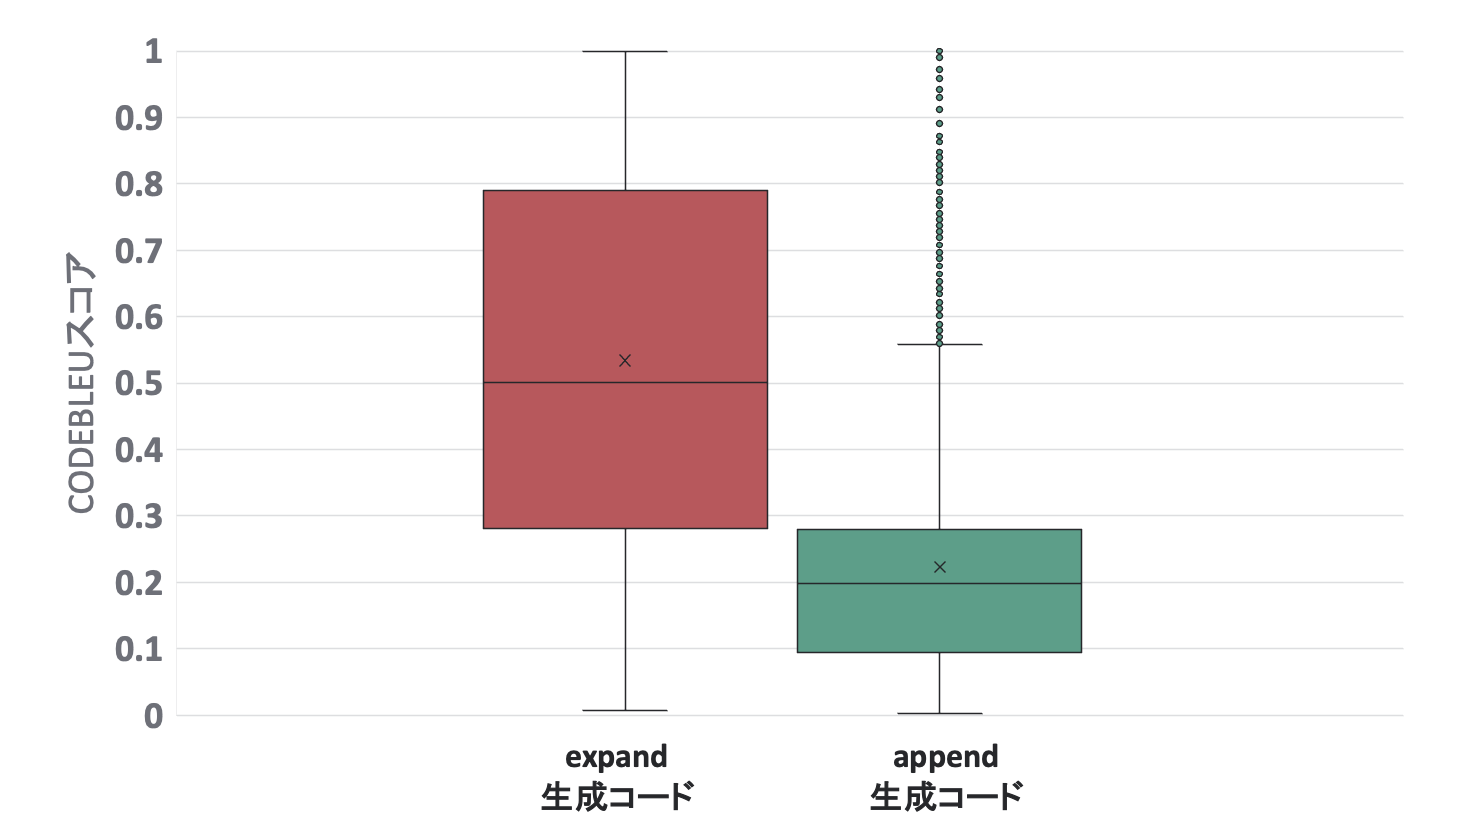
\includegraphics[width=0.9\linewidth]{@BSthesis2024_Akamatsu/Akamatsu_figs/rq2_result01.png}
\caption{GPTによる拡張の有無によるCodeBLEUスコアの比較}
\label{fig:boxplot}
\end{figure}

\subsection{結果2:スコアが上昇するような拡張コメントの特徴}
7,079件のレビューコメントペアに対して.CodeBLEUスコアと編集距離に基づくクラスタリング分析を実施した.クラスタ数の決定にはエルボー法を用い,k=4が最適であると判断した.また,初期クラスタ中心の選択にはk-means++を採用し,より安定したクラスタリング結果を得た.分析結果から,レビューコメントの拡張パターンは4つの特徴的なクラスタに分類された.


\begin{figure}[htbp]
\centering
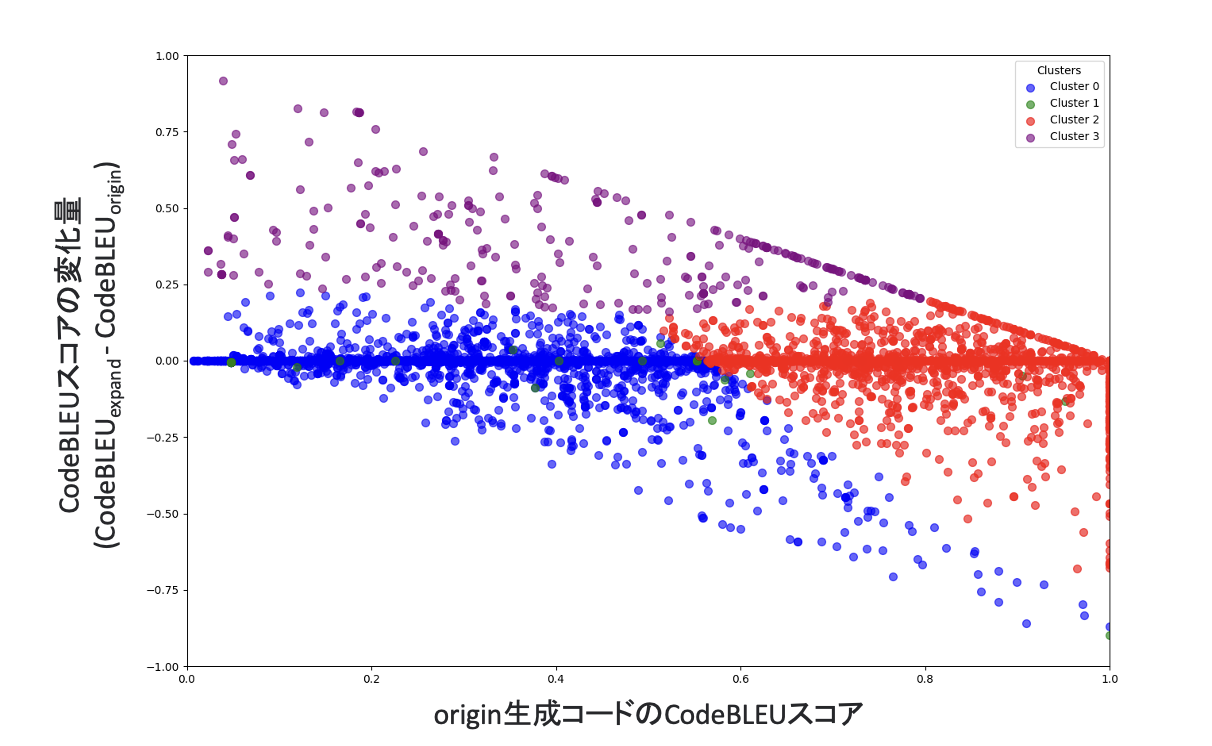
\includegraphics[width=0.9\linewidth]{@BSthesis2024_Akamatsu/Akamatsu_figs/rq2_result02_02.png}
\caption{元のCodeBLEUスコアとスコア変化量の関係}
\label{fig:scatter-cluster}
\end{figure}
図\ref{fig:scatter-cluster}は,横軸に元のCodeBLEUスコア,縦軸にスコアの変化量をとり,各データポイントをクラスタごとに色分けした散布図を示している.この図から,以下の4つの特徴的なクラスタの分布が確認できる.

\subsubsection{クラスタの基本特性}
クラスタ分析の結果, 4つの特徴的なグループが確認された. 低スコア安定グループ(クラスタ0)は図中の青色で示され, 3,784件のデータが低スコア領域(0.0-0.4)に集中している. このグループのスコアは0.312から0.294へと微減し, 編集距離は平均234.5文字であった. 大規模変更グループ(クラスタ1)は図中の緑色で示される31件の少数グループであり, 中程度のスコア領域(0.4-0.6)で大きな変動を示している. スコアは0.438から0.385へと低下し, 編集距離は平均2076.9文字と突出して大きい値を示した. 高スコア安定グループ(クラスタ2)は図中の赤色で示される2,962件のグループで, 高スコア領域(0.6-1.0)に分布している. スコアは0.830から0.816へと微減し, 編集距離は平均229.6文字であった. 改善成功グループ(クラスタ3)は図中の紫色で示される294件のグループで, 中程度のスコアから高スコアへの改善に成功している. このグループのスコアは0.432から0.798へと大幅に上昇し, 編集距離は平均231.7文字であった.
\subsubsection{効果的な拡張パターン}
散布図とクラスタ分析から, いくつかの効果的な拡張パターンが明らかになった. まず, メソッド名やクラス名などの具体的な技術要素を明示的に言及し, 関連するプロジェクトやコンポーネントについても説明を加えることで, スコアの向上が見られた. また, スコアが上昇したケースの多くは200-250文字程度の編集距離を維持しており, 2,000文字を超える大規模な変更は逆効果であることが示された. さらに, 元のスコアに応じた戦略の重要性も明らかになった. 元のスコアが0.4以下の場合は積極的な改善が効果的である一方, 0.8以上の高スコアの場合は最小限の修正に留めることが推奨される. 特に図\ref{fig:scatter-cluster}から, 元のスコアが0.4付近のデータポイントで大きな改善の余地があることが確認できた.

\subsubsection{改善成功グループの特徴}
特に注目すべき改善成功グループ(クラスタ3)では, いくつかの重要な共通点が観察された. まず, コードの具体的な部分を指摘し, その意図や目的を明確に説明することで, スコアの大幅な向上(平均+0.365)を実現している. また, 平均231.7文字という適度な長さを維持しながら, 必要な情報を過不足なく提供することで, 100\%の改善率を達成している. さらに, 変更による影響範囲やユーザーへの影響を具体的に説明することで, より効果的な拡張を実現している. 図\ref{fig:scatter-cluster}からも, このグループが一貫して正のスコア変化を示していることが確認できる.



\chapter{考察}\label{chap:fig-tab-exp}

\section{「具体的な修正方法の提示」のラベルが付いたコメントが付いていないコメントよりもスコアが高くなった要因}
本節ではRQ1の分析の結果,「具体的な修正方法の提示」のラベルが付いたレビューコメントがつかなったものに比べスコアが高くなった要因について事例をもとに考察する.

\begin{figure}[H]
   \begin{center}
       \fbox{\begin{minipage}{0.95\linewidth}
           CODEBLEU score: 0.5755\\
           \textbf{修正前コード:}\\
           
           \ttfamily\small
           private void handleMessage(Message message)\{\\
               try \{\\
                   \hspace{4ex}messageHandler.handleMessage(message);\\
                   \hspace{4ex}getSuccessCounter().increment();\\
                   \hspace{4ex}// 省略:メッセージ処理の後処理に関する複数行のコード\\
               \} catch (Exception e) \{\\
                   \hspace{4ex}log.error("failed to process message \{\}", message, e);\\
                   \hspace{4ex}getErrorCounter(e).increment();\\
               \}\\
           \}\\
           
           \normalfont\hrule
           
           \textbf{レビューコメント:}\\
           is messageHandler's job mark message handled successfully? sense put responsibility in here, error return message queue a failure status eventually get DLQ'd (otherwise redrive visiblity timeout expires - a longer backoff want)
       \end{minipage}}
       \caption{「具体的な修正方法の提示」以外のラベルが付いている事例}
       \label{fig:code-modification}
   \end{center}
\end{figure}

このレビューコメントは,メッセージの処理状態を適切に管理すべきことを示唆しているが,具体的な修正方法が示されていないため,以下のような複数の修正方法が考えられる:

\begin{itemize}
    \item メッセージの状態を追跡するための新しいクラスを作成する
    \item messageHandlerのインターフェースに成功/失敗のステータスを追加する
    \item 例外処理後にメッセージを再キューイングする
    \item Dead Letter Queue (DLQ)への移動処理を実装する
    \item try-catchブロックでメッセージの確認応答を制御する
\end{itemize}

このように修正方法が複数考えられる場合,自動修正モデルは必ずしもレビューアが意図した修正を生成できない.実際,このケースの修正後のコードでは,例外をキャプチャしてメッセージの確認応答(ack/nack)を制御する実装が採用されているが,これはレビューコメントから直接的に導き出すことが困難な実装である.このような複雑な修正の場合,具体的な修正方法を提示することが特に重要となる.

一方で,本研究の分析結果が示すように,具体的な修正方法を提示したレビューコメントでは,コンテキストの種類によらず一貫して高い精度を示している.これは,レビューアの意図する修正方法が明確に示されることで,モデルが適切な修正を生成できるためと考えられる.この結果は,コードレビューの実践において,問題点の指摘だけでなく具体的な修正方法を示すことの重要性を定量的に裏付けるものである.

\section{各クラスタにおけるレビューコメント拡張の特徴と改善効果の考察}

本節ではRQ2の分析の各クラスタの特徴をより明確にするため, 代表的な事例をもとに考察する. 図\ref{fig:success-case}, 図\ref{fig:failure-case}, 図\ref{fig:high-score-case}に, それぞれ改善成功事例, 悪化事例, 高スコア維持事例を示す.

\begin{figure}[h]
   \centering
   \fbox{\begin{minipage}{0.95\linewidth}
       \textbf{改善成功事例(クラスタ3)} \\
       \textbf{CODEBLEU score: 0.917 (0.039 → 0.956)} \\
       \textbf{編集距離: 203文字} \\
       
       \ttfamily\small
Before: \\
This override SHOULD not be included in the pull request, as it makes sense internally only.\\
\normalfont\hrule
After: \\
\ttfamily\small
The review comment indicates that the overridden method `getLmqQueueOffset` should not be included in the pull request because its functionality is considered internal to the codebase. This suggests that the method might not be relevant or necessary for external users or consumers.
   \end{minipage}}
   \caption{改善成功事例}
   \label{fig:success-case}
\end{figure}


\paragraph{改善成功事例(クラスタ3)}
図\ref{fig:success-case}に示す事例では, メソッド名(getLmqQueueOffset)を具体的に明示し, そのメソッドが内部利用に限定される理由を説明している. さらに, 外部ユーザーへの影響について言及しながら, 203文字という適切な長さで説明を完結させている. これらの要素が効果的に機能し, CodeBLEUスコアの大幅な向上(0.039から0.956)につながったと考えられる.


\begin{figure}[h]
   \centering
   \fbox{\begin{minipage}{0.95\linewidth}
       \textbf{大規模変更による悪化事例(クラスタ1)} \\
       \textbf{CODEBLEU score: -0.195 (0.569 → 0.374)} \\
       \textbf{編集距離: 1296文字} \\
       
       \ttfamily\small
Before: \\
I need to check the migration script, but I believe it might have compatibility issues with older versions. We should test it thoroughly.\\
\normalfont\hrule
After: \\
\ttfamily\small
The database migration script requires careful review and testing due to potential compatibility concerns. Specifically, when transitioning from versions prior to 2.x, the schema changes in the authentication tables might cause issues with existing user sessions and role mappings. A comprehensive test plan should include: 1) Verification of data integrity during the upgrade process, 2) Validation of existing user permissions and role assignments, 3) Testing of session management and token validation in mixed-version environments.
   \end{minipage}}
   \caption{悪化事例}
   \label{fig:failure-case}
\end{figure}


\paragraph{大規模変更による悪化事例(クラスタ1)}
図\ref{fig:failure-case}に示す事例では, 1296文字という過度に詳細な説明により文章が長大化している. また, データベースの移行スクリプトやスキーマ変更など, 具体的な技術要素への言及が文章全体に散在しており, 本質的な問題指摘が冗長な説明に埋没してしまっている. この結果, CodeBLEUスコアが0.569から0.374へと低下する結果となった.


\begin{figure}[h]
   \centering
   \fbox{\begin{minipage}{0.95\linewidth}
       \textbf{高スコア維持事例(クラスタ2)} \\
       \textbf{CODEBLEU score: 0.195 (0.805 → 1.000)} \\
       \textbf{編集距離: 196文字} \\
       
       \ttfamily\small
Before: \\
...so that it is now only used when dealing with subclass mappings. Might argue for possibly refining that.\\
\normalfont\hrule
After: \\
\ttfamily\small
The provided code snippet defines a method `forInheritance` in the `BeanMappingOptions` class. This method is designed to create a new `BeanMappingOptions` instance specifically for inheritance scenarios in bean mapping.
   \end{minipage}}
   \caption{高スコア維持事例}
   \label{fig:high-score-case}
\end{figure}

\paragraph{高スコア維持事例(クラスタ2)}
図\ref{fig:high-score-case}に示す事例では, クラス名(BeanMappingOptions)とメソッド名(forInheritance)を具体的に明示しながら, そのメソッドの目的を簡潔に説明している. 196文字という適切な長さを保ちながら必要な情報を過不足なく提供することで, 高いCodeBLEUスコア(0.805から1.000)を達成している.

これらの事例から, 効果的なレビューコメントの拡張には, 具体的な技術要素への言及, 適切な長さの維持, そして本質的な問題点の明確な説明が重要であることが確認できる. 特に, 編集距離を200-250文字程度に抑えながら, 必要な技術情報を過不足なく提供することが, 高いスコアの達成につながると考えられる.

\chapter{妥当性への脅威}\label{chap:fig-tab-exp}

\section{内的妥当性}

本研究の内的妥当性に関して,以下の3つの脅威が考えられる.

第一に,レビューコメントに対するラベル付けの主観性である.RQ1では,レビューコメントの情報の種類を「コンテキスト」と「修正依頼方法」という観点でラベル付けを行ったが,このラベル付けは研究者の主観的な判断に基づいている.1つのレビューコメントに複数の要素が含まれる場合,主たる情報の判断が研究者の解釈に依存する可能性がある.この脅威に対しては,複数の研究者による独立したラベル付けと,その一致度の評価を行うことで,より客観的な分析が可能となる.

第二に,GPTによるレビューコメントの拡張における一貫性の問題である.RQ2では,GPTを用いてレビューコメントの拡張を行ったが,大規模言語モデルの出力には一定の確率的な要素が含まれ,同じ入力に対しても異なる出力が生成される可能性がある.この非決定性が分析結果に影響を与える可能性がある.この脅威に対しては,各レビューコメントに対して複数回の拡張を試み,結果の安定性を確認する必要がある.

第三に,CodeBLEUスコアの評価指標としての妥当性である.本研究では,生成されたコードの品質をCodeBLEUスコアで評価しているが,このスコアが実際のコードの品質や意図した修正の正確さを完全に反映しているとは限らない.例えば,構文的には類似していても意味的に異なるコード修正が高いスコアを得る可能性がある.この脅威に対しては,人手による定性的な評価を併用することで,より包括的な評価が可能となる.

\section {外的妥当性}
本研究の外的妥当性に関して,以下の2つの制限事項が考えられる.

第一に,分析対象としたデータセットの特性による制限である.本研究では,GitHubにおいて多数のStarを獲得している大規模リポジトリを対象としている.これらのリポジトリでは,体系的なコードレビュープロセスが確立されており,レビューコメントの形式も一定の品質が保たれている可能性が高い.一方で,Star数の少ないリポジトリやより小規模なプロジェクトでは,レビューの形式や厳密さが異なる可能性がある.そのため,本研究で得られた知見が,そのような環境下でも同様に適用できるかどうかは不明確である.

第二に,プログラミング言語の制約による制限である.本研究ではJavaを対象言語として分析を行っているが,他のプログラミング言語ではコーディング規約やベストプラクティスが異なり,それに伴いレビューの観点や方法も変化する可能性がある\cite{Berger2019On}.例えば,動的型付け言語では型に関する指摘が少なくなる一方で,実行時の動作に関する指摘が増える可能性がある.また,関数型言語では,オブジェクト指向とは異なるパラダイムに基づくレビュー指摘が行われる可能性がある.そのため,本研究の結果を他のプログラミング言語に直接適用することには慎重な検討が必要である.

\chapter{おわりに}

本研究では,コードレビューコメントの特徴がソースコードの自動修正精度に与える影響を分析するため,2つのRQを設定して調査を行った:

\begin{itemize}
\item RQ1:\RQone
\item RQ2:\RQtwo
\end{itemize}

RQ1では,レビューコメントの情報の種類を「コンテキスト」と「修正依頼方法」の2つの観点から分析した.その結果,修正の種類(リファクタリング,バグ修正,パフォーマンス改善)による精度の違いは限定的である一方,具体的な修正方法を提示するレビューコメントが最も高い精度を示すことが明らかになった.

RQ2では,GitHubのPull Request情報を用いてレビューコメントを拡張し,情報量と自動修正の精度の関係を分析した.結果,GPTを用いて200-250文字程度の適切な長さに拡張したレビューコメントが最も効果的であり,特に具体的な技術要素への言及を含む拡張が精度向上に寄与することが示された.

ソフトウェア開発の現場では,コードレビューの効率化が重要な課題となっている.特に,レビューアの意図を正確に実装者に伝え,適切な修正を実現することは,開発の生産性と品質に大きく影響する.本研究では,レビューコメントから自動的にコード修正を生成する際に,どのような情報が必要であり,どの程度の情報量が適切かを明らかにした.これらの知見は,効果的なレビューコメントの作成指針として活用できる.

今後の課題として,以下の2点が挙げられる.第一に,より多様なプログラミング言語やプロジェクト規模での検証である.本研究ではJavaを対象としたが,他の言語でも同様の結果が得られるか検証する必要がある.第二に,レビューコメントの自動拡張の改善である.GPTによる拡張の精度をさらに向上させるため,プロジェクト固有の文脈や開発履歴を考慮した拡張手法の提案が考えられる.


\begin{acknowledgements}
研究活動に取り組むにあたって多くの方々に御指導,御協力を賜りました.ここに御世話になった方々への感謝の意を記させていただきます.

指導教員である和歌山大学システム工学部伊原彰紀准教授に対し,厚く御礼申し上げます.研究室に配属して以来,研究方針についての相談,論文執筆,発表資料制作など多くの時間を割いて御指導をしていただきました.特に,学生である私に対しても妥協することなく,丁寧かつ熱心な御指導をいただきました.また,学会発表の機会を多くいただき,自分の見識を広めることができました.先生の御尽力に敬意を表し,心より感謝いたします.

また,和歌山大学ソーシャルソフトウェア工学研究室の方々には,研究に関する客観的な御意見や御指摘を常日頃から数多くいただきました.心より感謝いたします.

最後に,常に私を励まし,支えてくれた家族に,心より感謝します.

\end{acknowledgements}


%%
%% 参考文献
%%
\bibliographystyle{junsrt}
\bibliography{@BSthesis2024_Akamatsu/BSthesis2024_Akamatsu}

%%%%%%%%%%%%%%%%%%%%%%%%%%%%%%%%%%%%%%%%%%%%%%%%%%%%%%%%%%%%%%%%%%%%%%%%

%%
%% 付録
%%
% \appendix
% 
% \chapter{サンプルプログラム}
% 
% プログラムリストや実行結果など,本論を補足する上で必要と思われるものが
% あれば付録として付ける.
% 
% {
% \footnotesize
% \begin{verbatim}
% #include <stdio.h>
% int main(void)
% {
%     printf("Hello, World!\n");
%     return 0;
% }
% \end{verbatim}
% }

%%%%%%%%%%%%%%%%%%%%%%%%%%%%%%%%%%%%%%%%%%%%%%%%%%%%%%%%%%%%%%%%%%%%%%%%

\end{document}
